\chapter{Attentive Guidance}\label{Chapter:proposals}

In this chapter I introduce the concept of \textbf{Attentive Guidance (AG)} which is a novel mechanism to equip seq2seq models with an additional bias to nudge them in the direction of finding a compositional solution from the search space of all possible solutions. This chapter begins with a brief overview of the prime motivation for my proposal, followed by the details of attentive guidance. I conclude my discussion on AG by showing how attentive guidance relates to the concept of pondering that we saw in section \ref{bck:ponder}. This chapter then introduces two datasets which serve as testbeds for attentive guidance. I motivate the relevance of these datasets as pertinent test regimes for attentive guidance followed by the experimental setup for both a vanilla seq2seq baseline and an attentive guidance model. I conclude with the results obtained and a comparative analysis of vanilla seq2seq and attentive guidance on each of these domains.

%(models capable of zero shot generalizing to unseen inputs on known compositions). Additional these small percentage of models also only showed a weak form of composition wherein if for instance t1, t2 are atomic tables, then a composition task t1 t2 is indexed to prompt t1t2, instead of solving in a nested fashion viz. t1(t2(.)). (Get feedback here, see if this is clear)

\section{Attentive Guidance}
Human beings have a propensity for compositional solutions \citep{NIPS2016_6130} while deep neural networks lean towards pattern recognition and memorization \citep{Marcus2018}. It is therefore reasonable to assume that for human level generalization learning in a systematic way is of essence. Attentive guidance aims to induce systematic learning in seq2seq networks by allowing them to focus on the primitive components of a complex expression and the way they are related to each other. The following sections elaborate on the motivation behind attentive guidance and its implementation.

\subsection{Inspiration} 

\cite{Lake2015} introduced Hierarchical Bayesian Program Learning (HBPL) to learn complex characters (concepts) from few samples by representing them as probabilistic programs which are built compositionally via. Bayesian sampling from simpler primitives, subparts, parts and the relations between them, respectively. This approach led to human level generalization on the \textbf{omniglot} dataset \citep{Lake2015} which is a dataset containing 1623 characters (concepts) with 20 samples each. Omniglot is therefore not sample intensive and hence ideally suited to test one-shot generalization capabilities of a model. This work served as the major motivation for learning nested functions such as \textit{lookup tables} (section \ref{datasets:lt}) of the form t1(t2(.)), by learning the compositions from simpler primitives i.e. atomic tables and then stacking them hierarchically. The procedure for learning the \textbf{trace} of the above-mentioned lookup table task is described subsequently.

\subsection{Implementation}

Attention (section \ref{mtv:attn}) based seq2seq models produce a \lq soft{}\rq\ alignment between the source (latent representation of the input) and the target. Furthermore seq2seq models require thousands of samples to learn this soft alignment. However in light of the aforementioned arguments presented in favor of concentrating on primitives to construct a complex \lq composition{}\rq\ I propose the concept of \textbf{A}ttentive \textbf{G}uidance (AG). AG argues that the decoder having perfect access to the encoder state(s) containing maximum information pertaining to that decoding step, would lead to improved target sequence accuracy.

%\begin{figure}
%	\begin{minipage}[t]{\textwidth}
%		\ifpdf
%		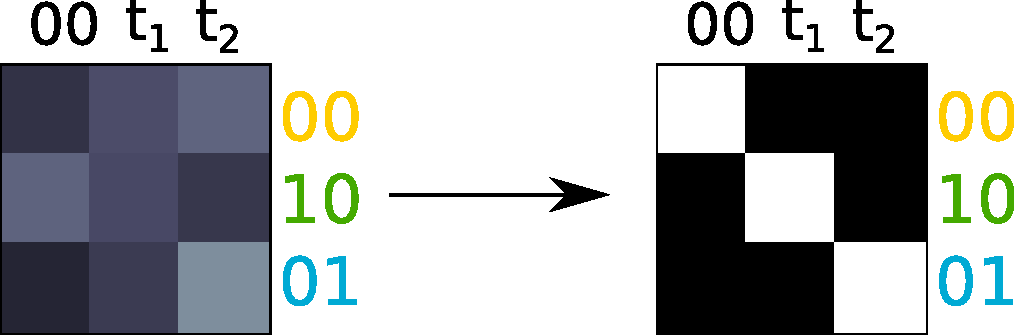
\includegraphics[width=\linewidth,keepaspectratio=true]{./figs/attention-guidance-pdf}
%		\else
%		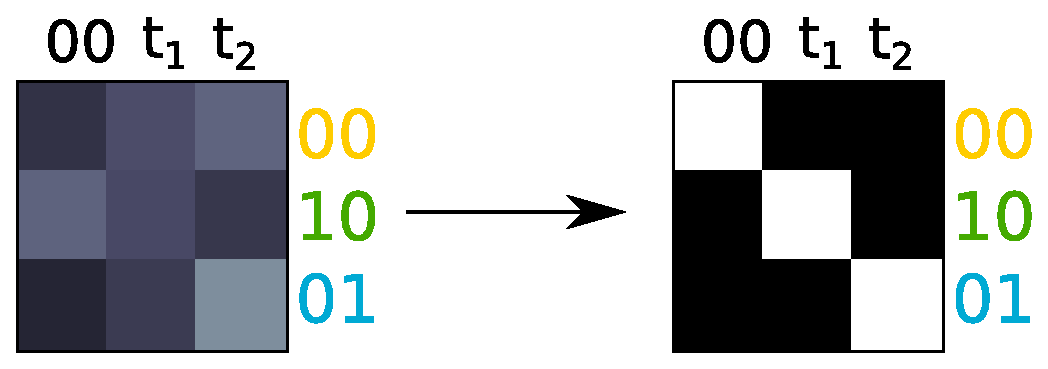
\includegraphics[width=\linewidth,keepaspectratio=true]{./figs/attention-guidance-eps}
%		\fi
%		\caption{\small Diffused vs Hard Attention}
%		\label{pm:ag-schematic}
%	\end{minipage}
%\end{figure}

Revisiting the query-key-value triplet view of attention described in section \ref{mtv:attn}, AG tries to improve the scalar matching score between the query and the keys during the attentive read step. Since the \textit{keys} can be thought of as the memory addresses to the \textit{values} which are needed at a given decoding step, AG tries to ensure a more efficient information retrieval. Similar to \cite{Lake2015} AG induces the trace of a program (although not probabilistic) needed to solve a complex composition by solving its subparts in a sequential and hierarchical fashion. This in turn forces the model to search for a compositional solution from the space of all possible solutions. AG eventually results in a \lq hard{}\rq\ alignment between the source and target.
%as seen in figure \ref{pm:ag-schematic}


\begin{figure}
	\begin{minipage}[t]{\textwidth}
		\ifpdf
		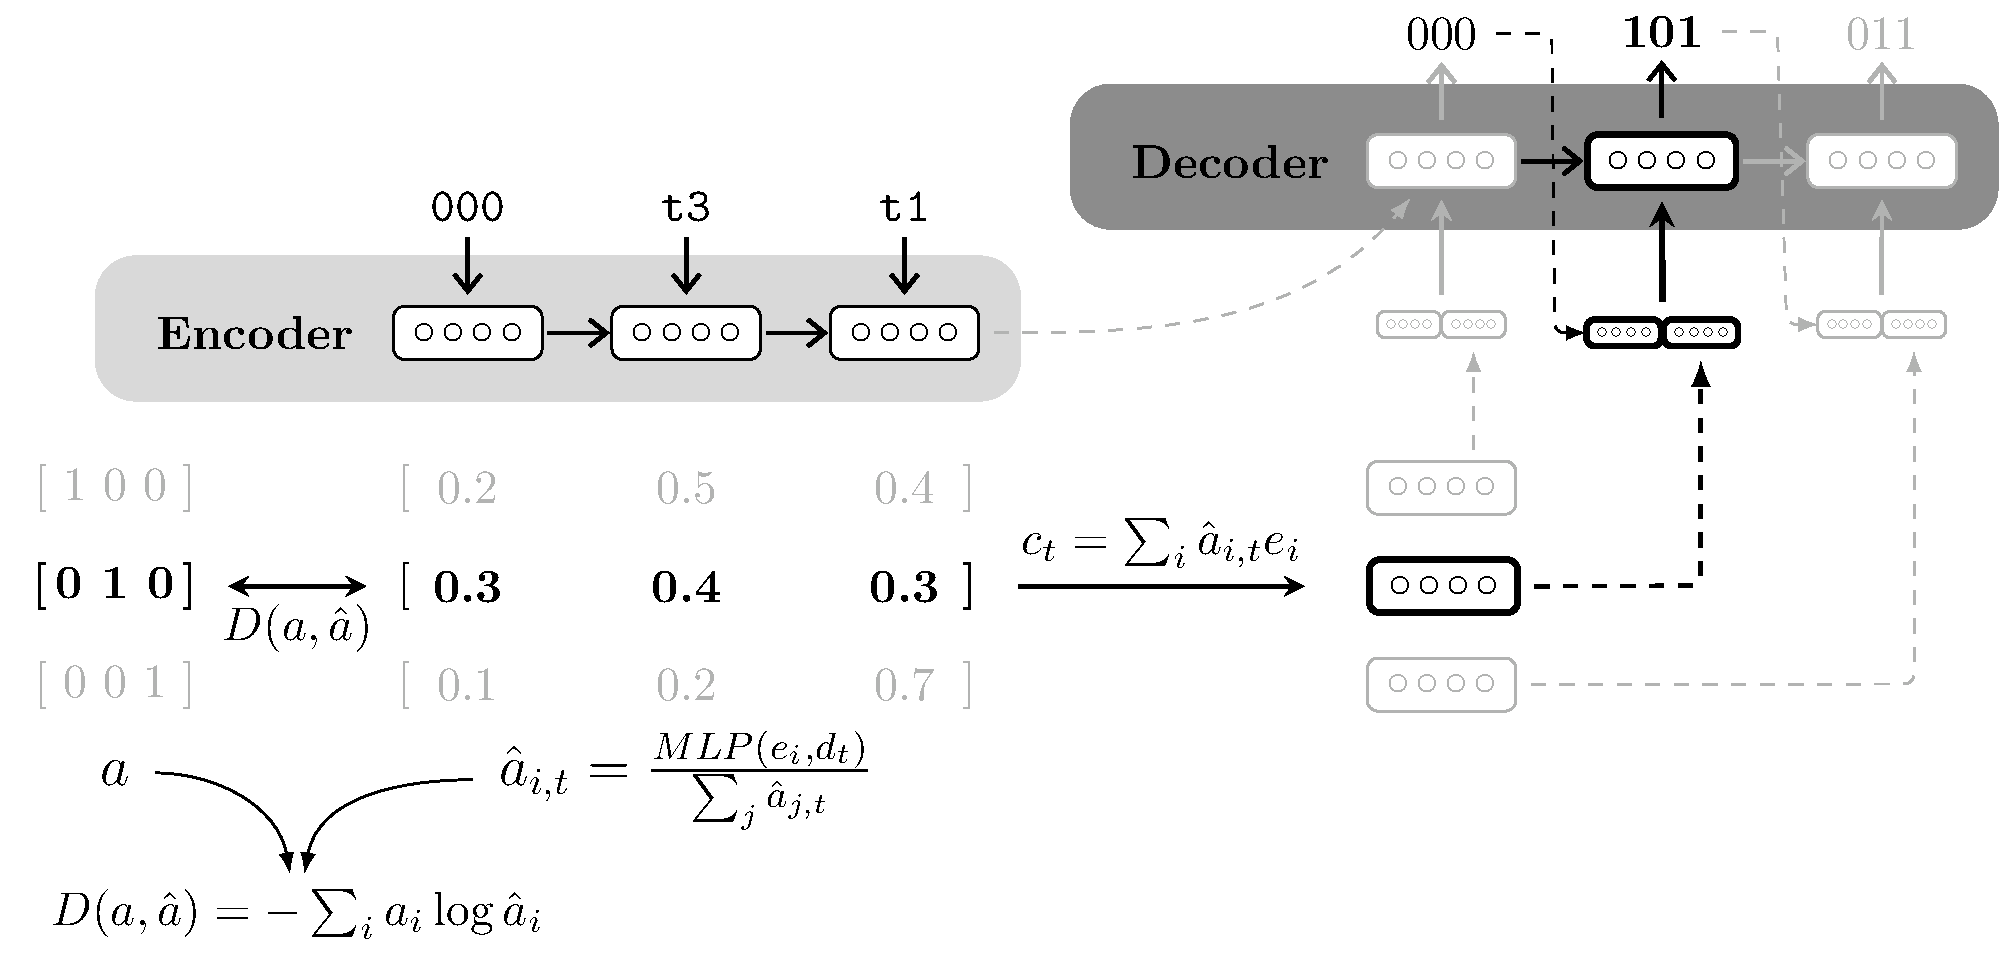
\includegraphics[width=\linewidth,keepaspectratio=true]{./figs/ag-model-pdf}
		\else
		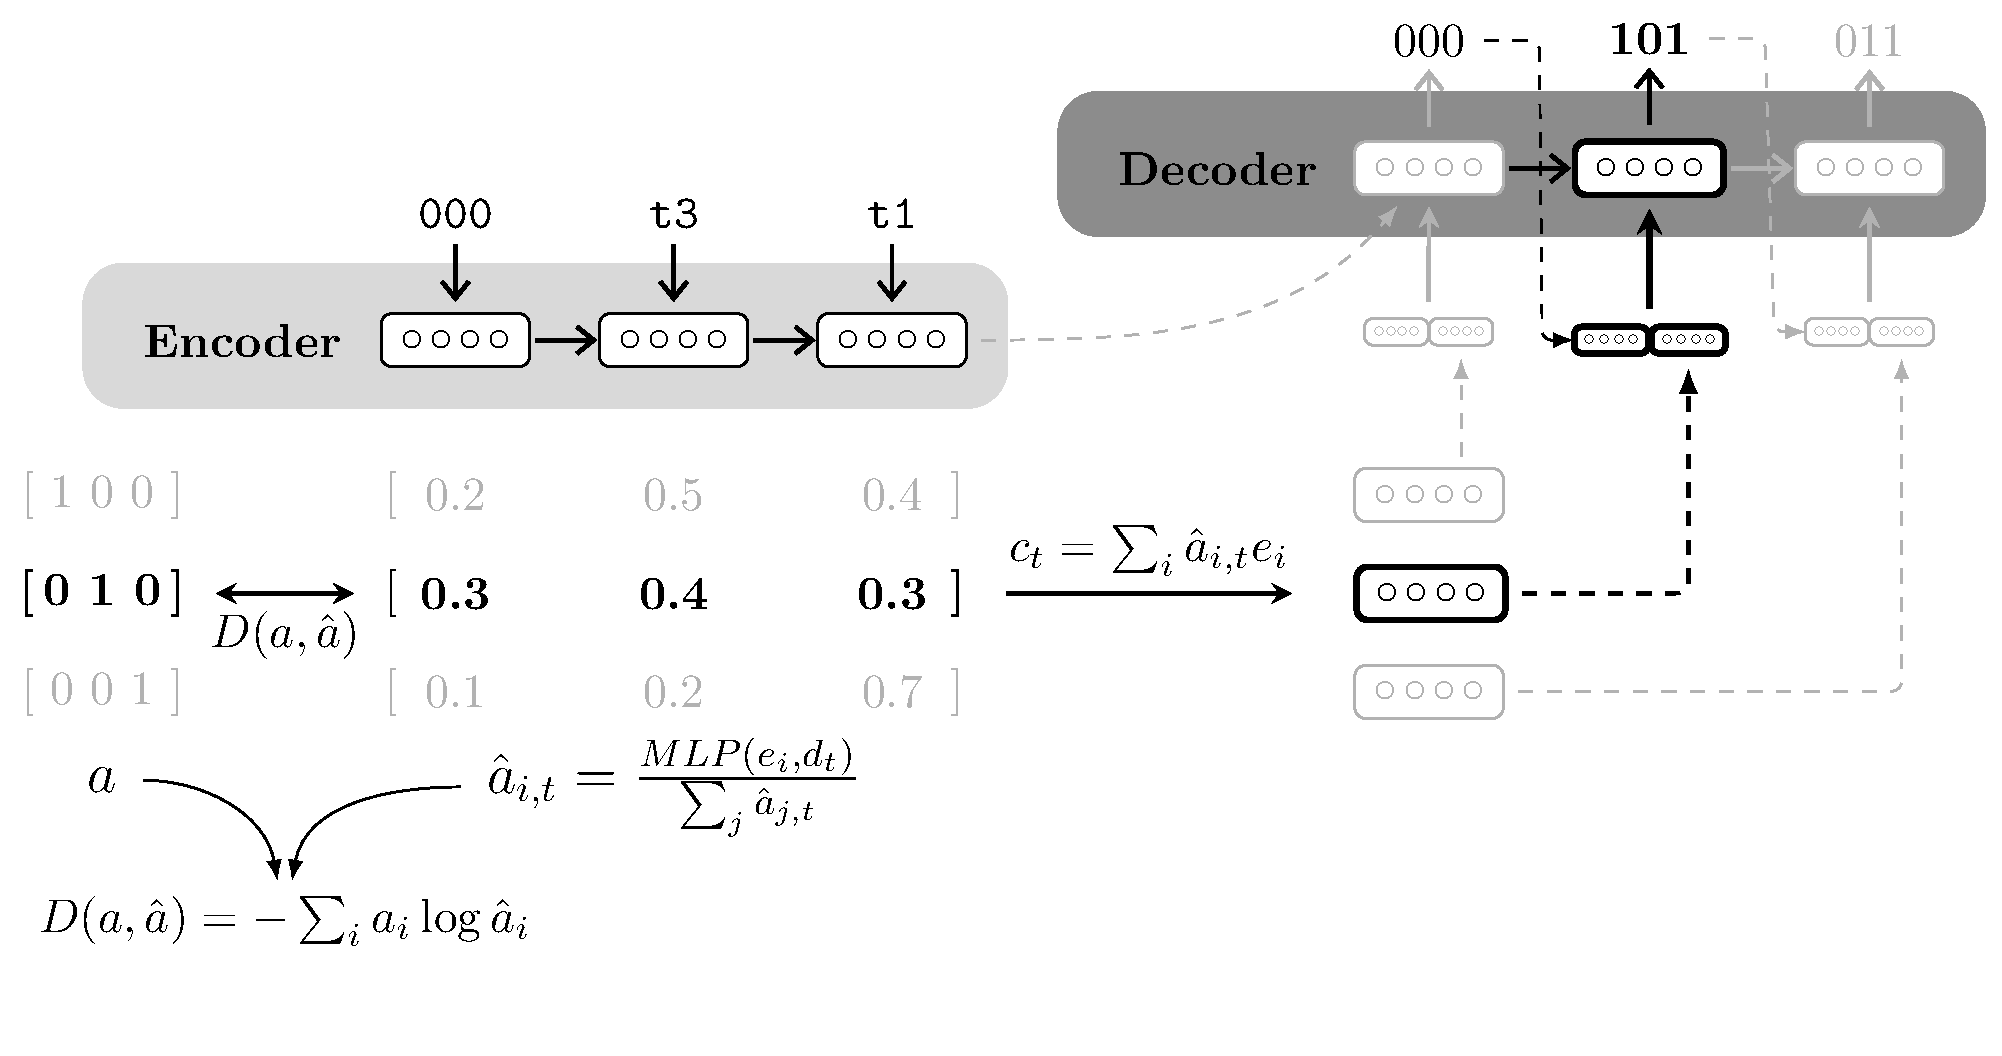
\includegraphics[width=\linewidth,keepaspectratio=true]{./figs/ag-model-eps}
		\fi
		\caption{\small Attentive Guidance and calculation of AG loss \citep{Hupkes2018}}
		\label{pm:ag-loss}
	\end{minipage}
\end{figure}

AG is implemented via an extra loss term added to the final model loss. As shown in figure \ref{pm:ag-loss}, at each step of decoding, the cross entropy loss between calculated attention vector $\hat{a}_{t,i}$ and the ideal attention vector $a_{t,i}$, are added to the model loss. The final loss for an output sequence of length $T$ and an input sequence of length $N$ is therefore expressed as:

\begin{equation}\label{eqn:ag}
\widetilde{\mathcal{L}}(x,y) = \mathcal{L}(x,y) + \sum_{t=1}^T \sum_{i=1}^N -a_{i,t}\log\hat{a}_{i,t}
\end{equation}

\subsection{AG and Pondering} \label{pm:ag-ponder}
Pondering presented in section \ref{bck:ponder} facilitates variable hidden state transitions at any given input step in a recurrent unit. Attentive guidance can be seen as hardcoded or forced pondering in case of seq2seq models. This is best elaborated through an example as follows:
\begin{equation}
	f(5) = 10 \qquad g(3) = 5\qquad f(g(3)) = 10,
\end{equation}
rewriting the composed function as follows and expanding each step of composition:
\begin{equation}
	f\ g\ 3 = 5\ 10.
\end{equation}
It is easy to see that if the above example is presented to a model all it needs to do is emit the final output i.e. 10. However AG forces an additional (ponder) step to explicitly emit the intermediate output as well. Not only does this allow the decoder of the output to have an additional hidden state transition it also helps us see if the model is taking compositional steps in arriving at the final answer. In this thesis I use such \lq mocked\rq{} pondering in case of lookup-tables (section \ref{datasets:lt}) and micro tasks (chapter \ref{Chapter:datasets}). As a future work we can think about coming up with a method to ensure that the number of ponder steps are learned by the decoder instead of being hardcoded.

\section{Lookup Tables} \label{datasets:lt}

The lookup tables task was introduced by \cite{Liska2018} within the CommAI domain \citep{Baroni2017} as an initial benchmark to test the generalization capability of a compositional learner. The data consists of atomic tables which bijectively map three bit inputs to three bit outputs. The compositional task can be understood in the form of a nested function $f(g(x))$ with $f$ and $g$ representing distinct atomic tables. To clarify the task with an example, given $t1$ and $t2$ refer to the first two atomic tables respectively; also given that $t1(001) = 100$ and $t2(100) = 010$. Then a compositional task is presented to a learner as $001\ t1\ t2 = 010$. Since the i/o strings are three bit, there can be a maximum of 8 input/output strings.

As is clear from the task description that since the table prompts $t_i$ don't have any semantic meaning in itself, the meaning of each individual table prompt can be correlated only with the bijective mapping it provides. Secondly the dataset is in agreement with the systematic compositionality definition that we have outlined in section \ref{systematic}. Lastly one can argue that even a human learner might come up with an approach that is different than solving each function individually and sequentially in a given nested composition, but such an approach will not be able to scale with the depth of nesting.

\cite{Liska2018} in their experiments with lookup tables found that by having additional supervision on the weights of hidden state transitions, theoretically a finite-state automata (FSA) can be induced such that the recurrent layers encode the states of this automaton. This FSA can in principle solve the lookup table task upto a finite number of compositions. They further showed that this theoretical setup can achieve zero state generalization on unseen inputs on known compositions i.e. \textit{heldout inputs} (section \ref{lt:splits}). However when trained purely on input/output mappings without this additional supervision, the authors noted that only a small percentage of networks could converge to a compositional solution.

%using lookup tables (section \ref{datasets:lt}) as the testbed tried to asses the ability of a RNN network (more specifically a 60 unit LSTM followed by a 10 unit sigmoid layer) to search for compositional solution to the lookup table task. Lookup tables exhibit functional nesting and therefore a model that can find a compositional solution from the search space of all possible solutions is more likely to zero shot generalize to novel compositions. The authors established that

\subsection{Data Structure}\label{lt:splits}
I generated eight distinct atomic tables $t1......t8$ and work with compositions of length two, i.e. $t_i - t_j$. This leads to a possible 64 compositions. Since the requirement for the model is to not simply memorize the compositions but rather to land on a compositional solution, I propose to use the compositions only from tables $t1 - t6$ for the training set. However, since the model needs to know the mapping produced by tables $t7, t8$ in order to solve their compositions we expose the model to the atomic tables $t7, t8$ in the training set. The details of all the data splits and some dataset statistics are presented below. Examples from each split and the size of each split are presented in table \ref{lt:stats}

\begin{enumerate}
	\item \textbf{train} - The training set consists of the 8 atomic tables on all 8 possible inputs. The total compositions of tables $t1 - t6 = 36$. Out of those 36 compositions we take out 8 compositions randomly. For the remaining 28 compositions we take out 2 inputs such that the training set remains balanced w.r.t. the compositions as well as the output strings. The algorithm for creation of this balanced train set is presented in appendix \ref{Chapter:results}.
	\item \textbf{heldout inputs} - The 2 inputs taken out from the 28 compositions in training constitute this test set. However of the 56 data points, 16 are taken out to form a validation set. In creating this split I ensured that the splits i.e. \textit{heldout inputs} and \textit{validation} have a uniform distribution in terms of output strings at the expense of the uniformity in the compositions.
	\item \textbf{heldout compositions} - This set is formed by the 8 compositions that were taken out of the initial 36 compositions. These 8 compositions are exposed to all 8 possible input strings.
	\item \textbf{heldout tables} - This test is a hybrid of the tables which are seen in compositions during training i.e. $t1 - t6$ and those which are seen just atomically during training i.e. $t7 - t8$. There are total of 24 compositions in this split which are exposed to all 8 inputs.
	\item \textbf{new compositions} - This split consists of compositions of $t7 - t8$ and therefore a total of 4 compositions on 8 inputs.
\end{enumerate}


\begin{table}[ht]
	\centering
	\begin{tabular}{l|lc}
		& Example & Size\\
		\hline
		train & t1 t2 011 & 232 \\
		heldout inputs & t1 t2 001 & 40 \\
		heldout compositions & t1 t3 110 & 64 \\
		heldout tables & t1 t8 111 & 192 \\
		new compositions & t7 t8 101 & 32 \\
	\end{tabular}
	\caption{Lookup Table Splits}
	\label{lt:stats}
\end{table}


\begin{figure}[ht]
	\begin{subfigure}{0.5\linewidth}
		\ifpdf
		\includegraphics[width=0.95\linewidth]{./figs/lookup/train-pdf}
		\else
		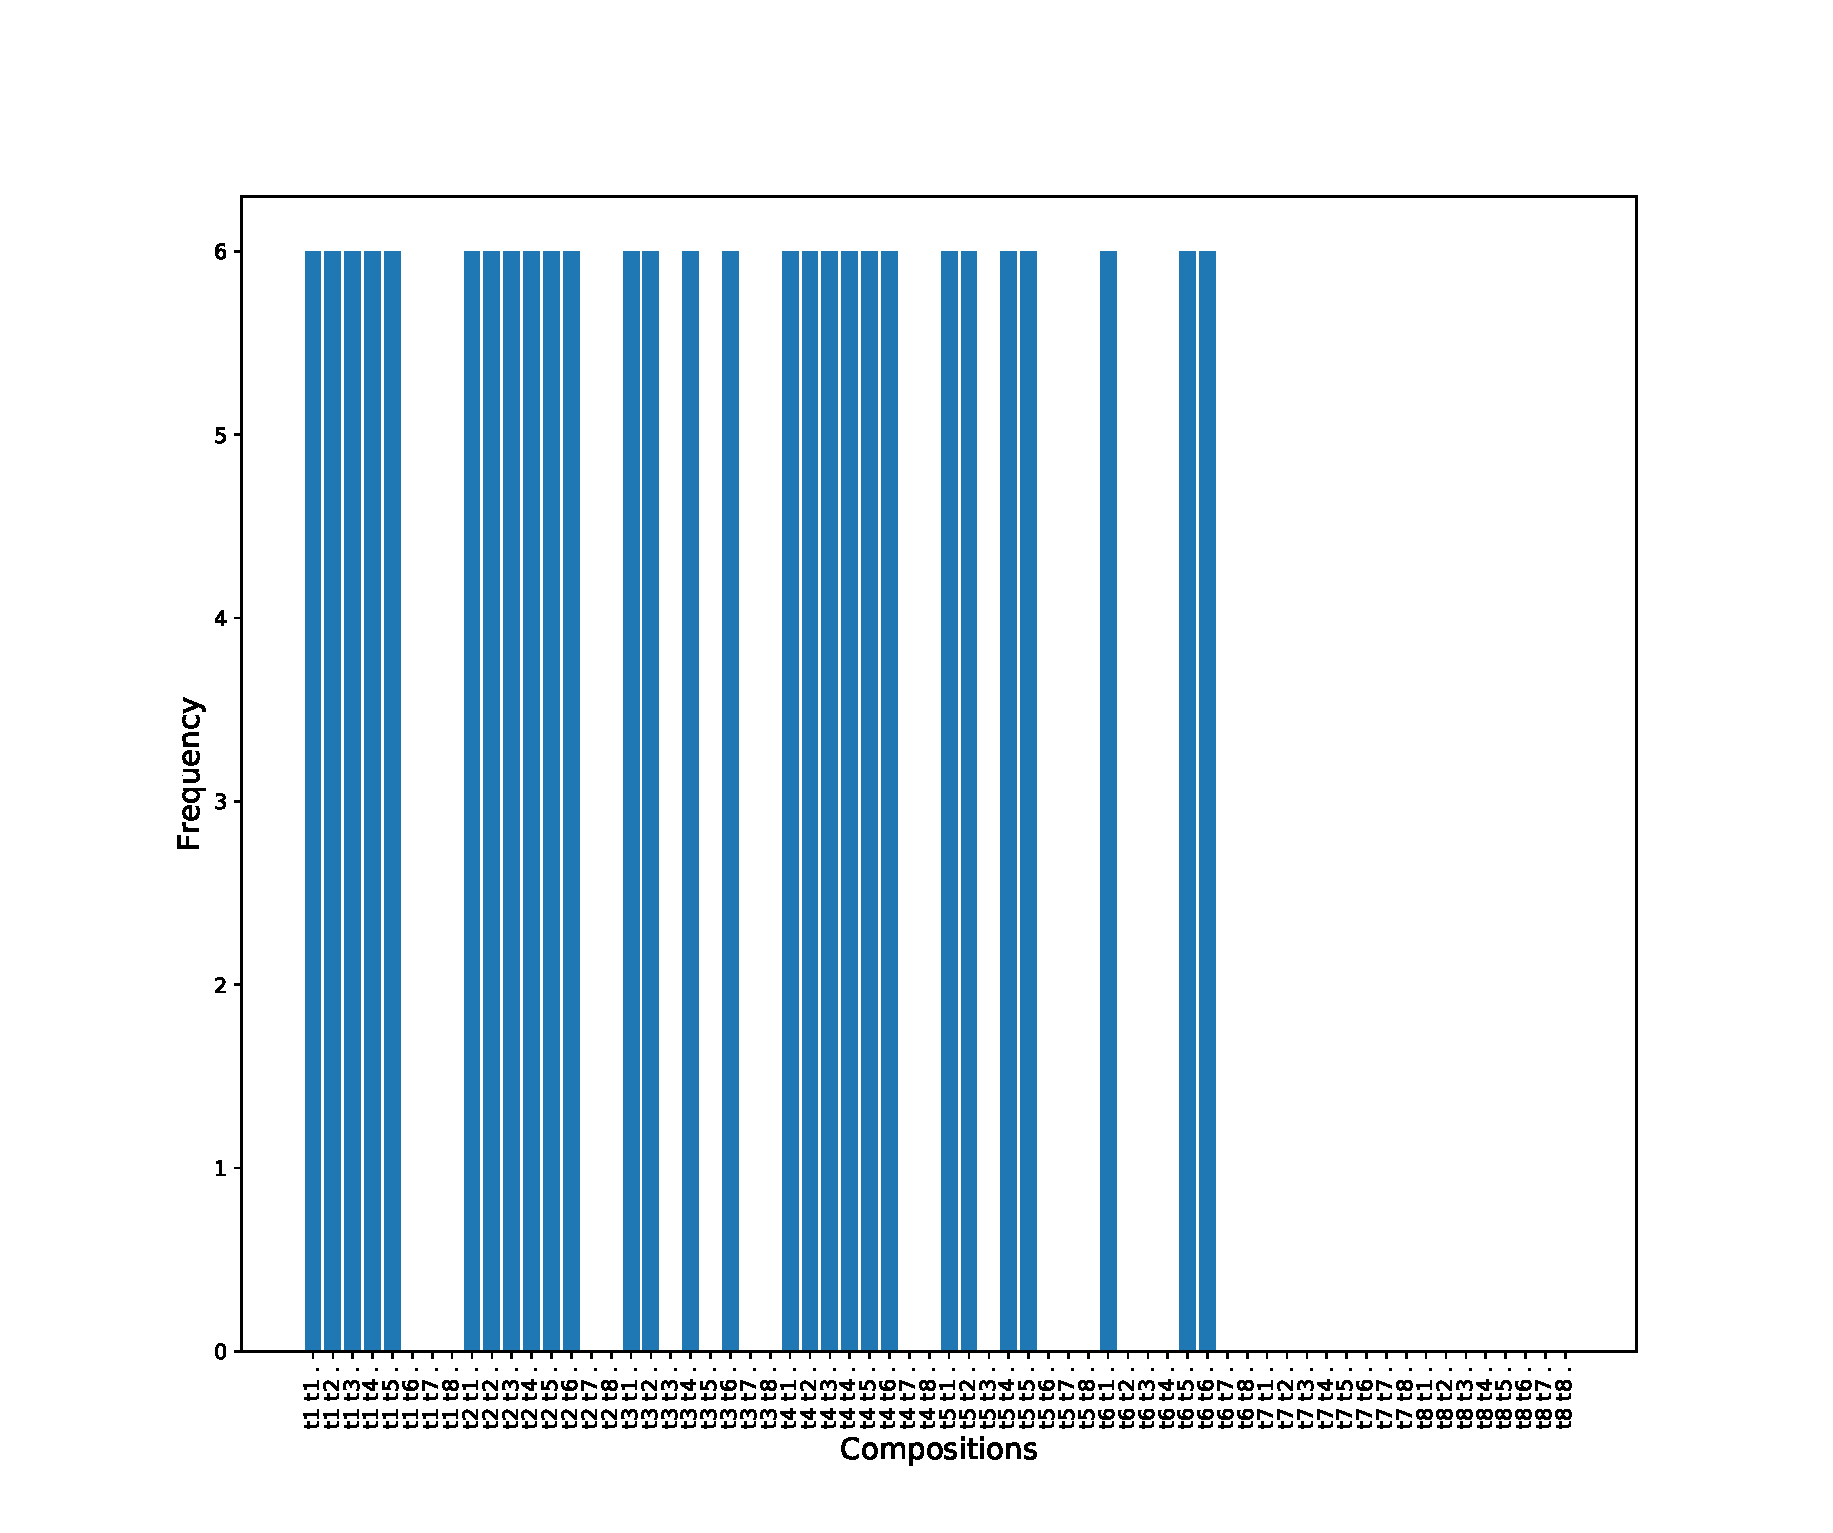
\includegraphics[width=0.95\linewidth]{./figs/lookup/train-eps}
		\fi
		\caption{Train}\label{fig:train_dist}
	\end{subfigure}
	\begin{subfigure}{0.5\linewidth}
		\ifpdf
		\includegraphics[width=0.95\linewidth]{./figs/lookup/heldout_compositions-pdf}
		\else
		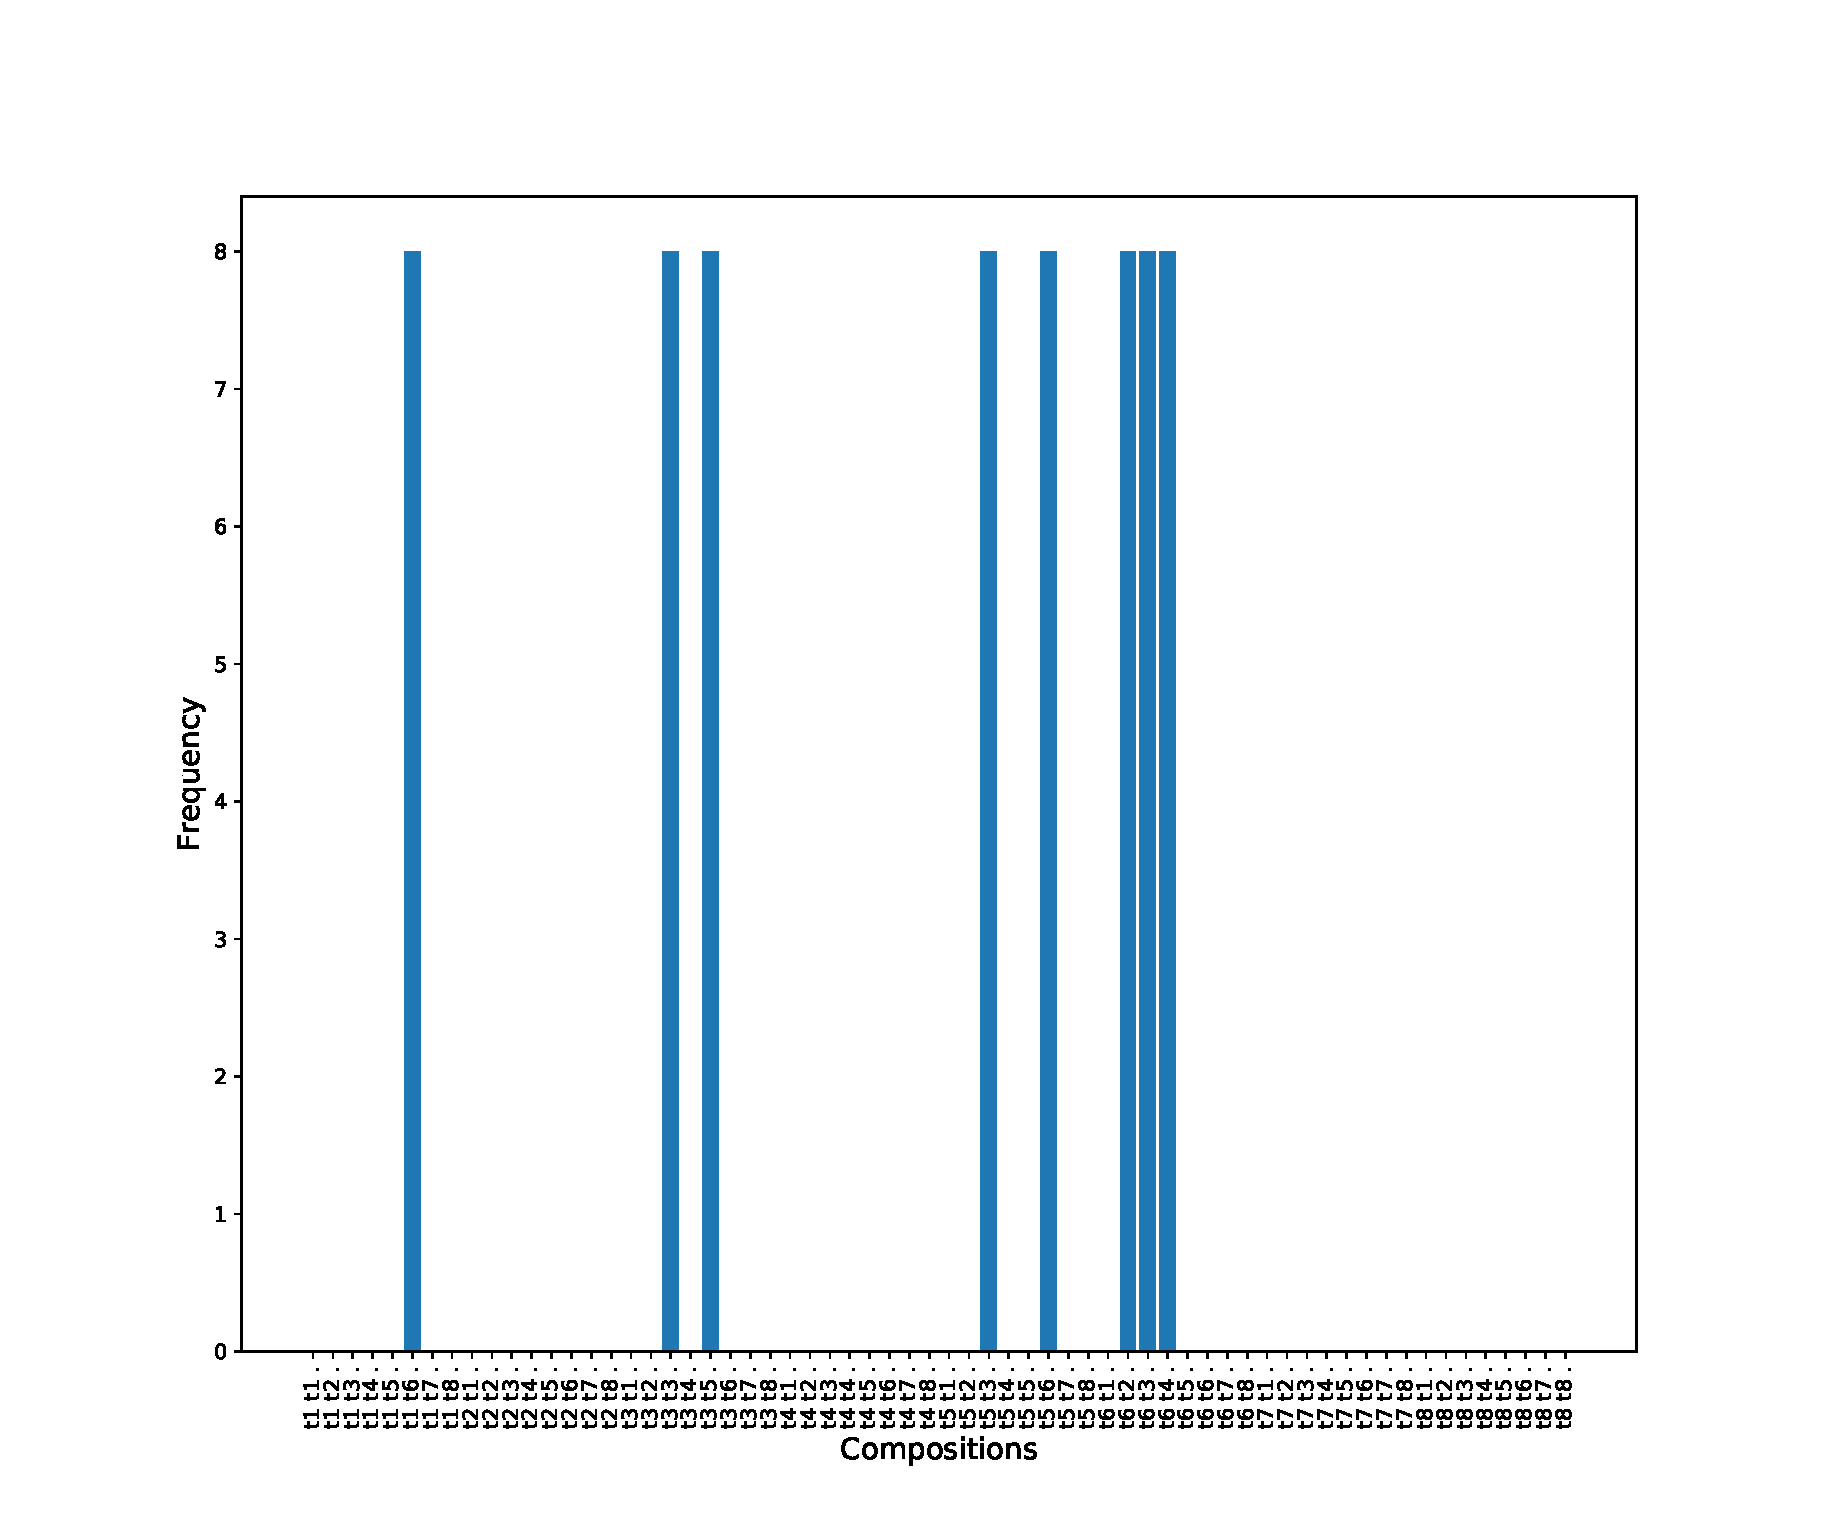
\includegraphics[width=0.95\linewidth]{./figs/lookup/heldout_compositions-eps}
		\fi
		\caption{Heldout Compositions}\label{fig:held_comp}
	\end{subfigure}
	\begin{subfigure}{0.5\linewidth}
		\ifpdf
		\includegraphics[width=0.95\linewidth]{./figs/lookup/heldout_tables-pdf}
		\else
		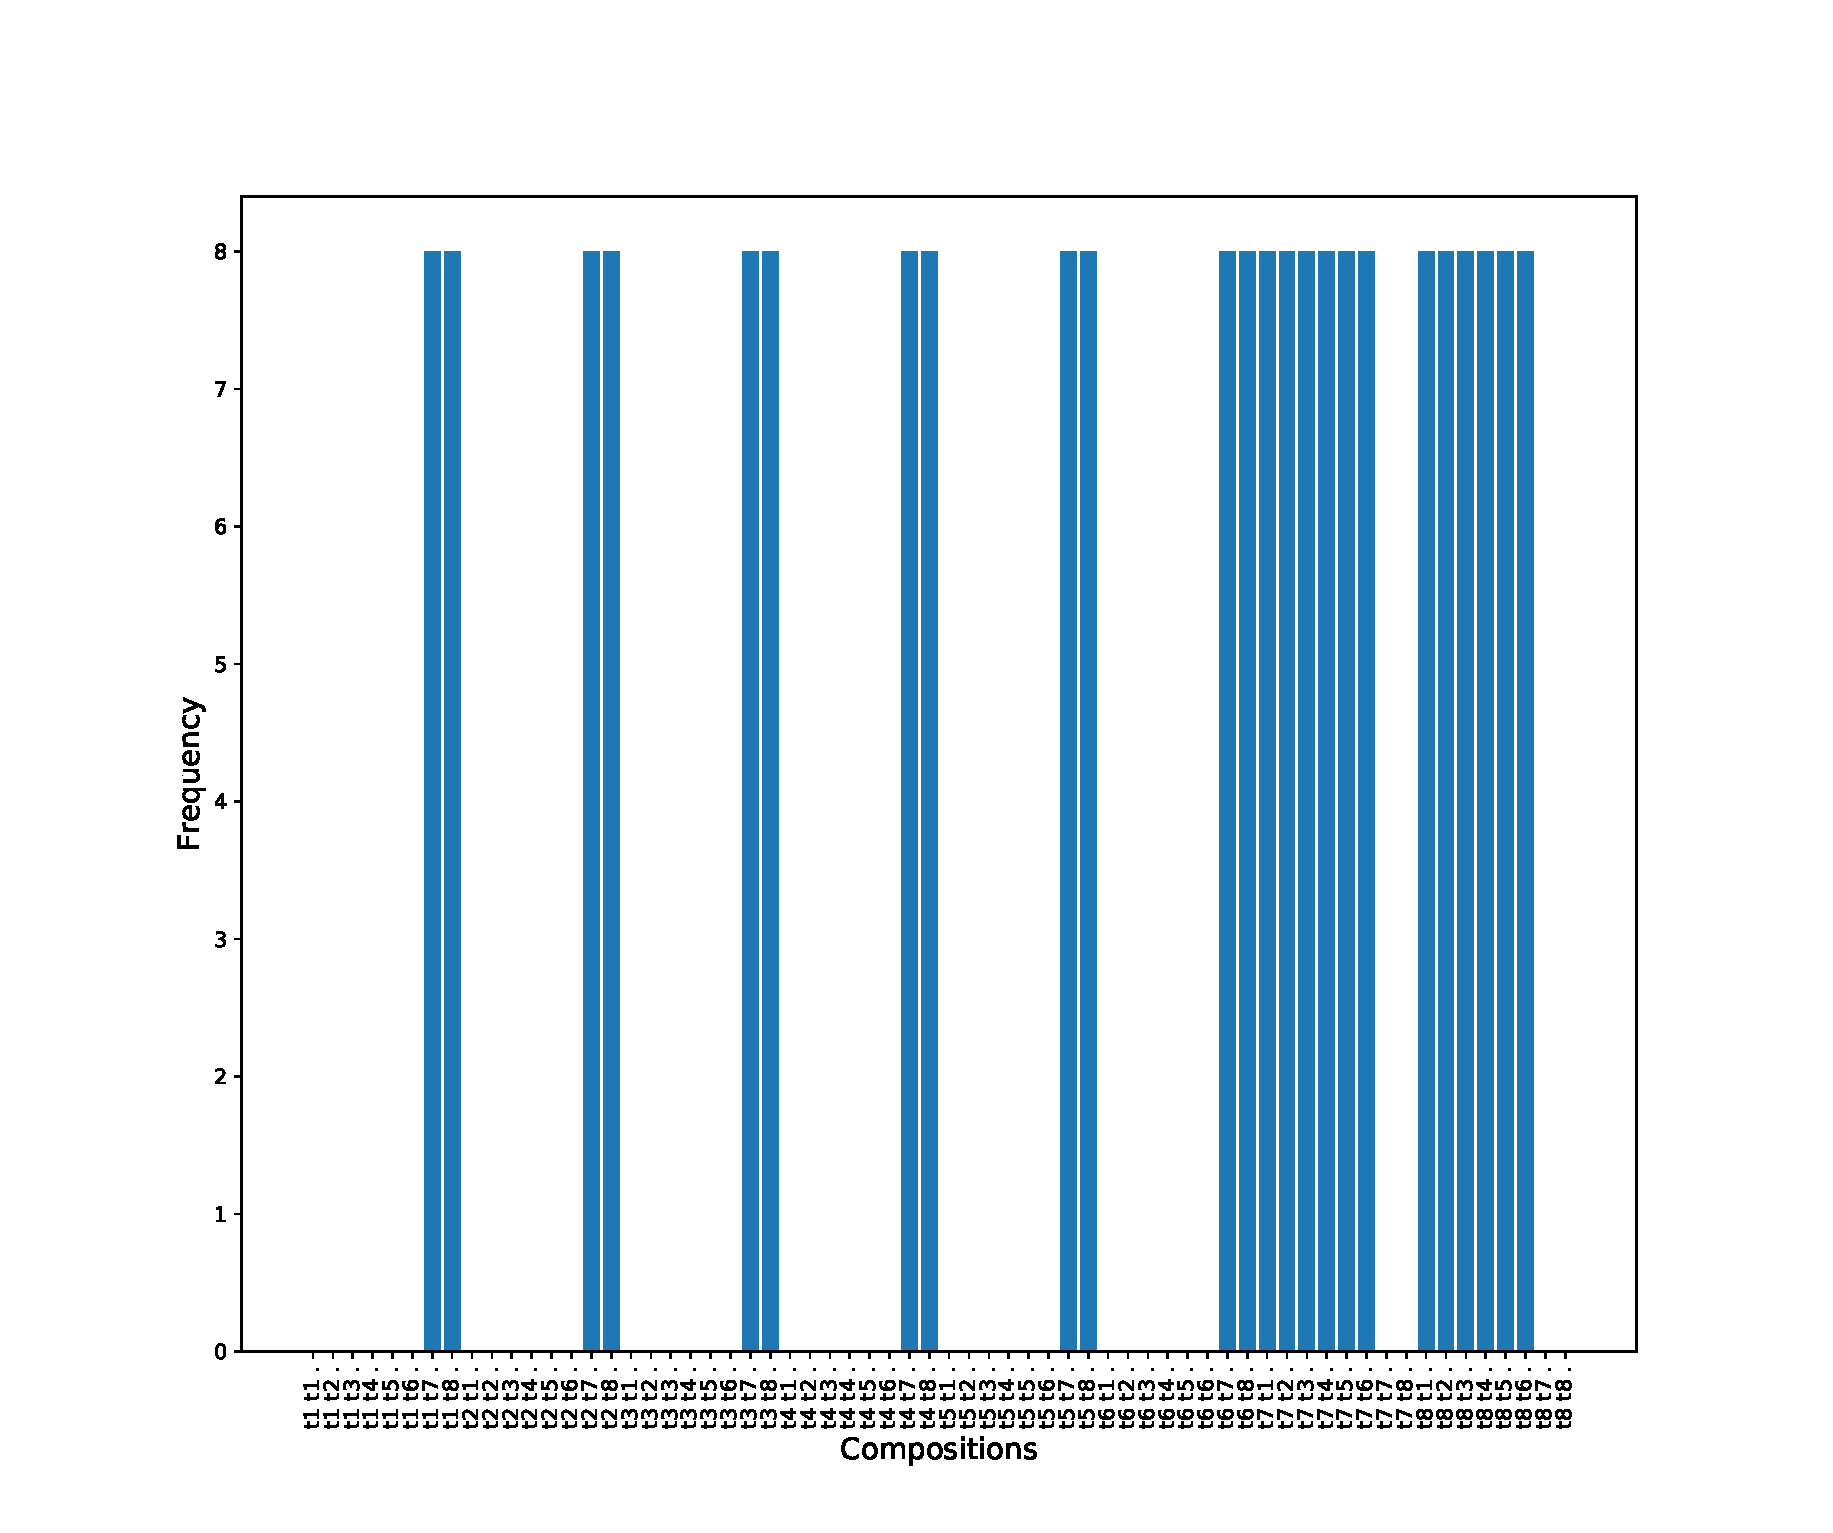
\includegraphics[width=0.95\linewidth]{./figs/lookup/heldout_tables-eps}
		\fi
		\caption{Heldout Tables}\label{fig:held_tab}
	\end{subfigure}
	\begin{subfigure}{0.5\linewidth}
		\ifpdf
		\includegraphics[width=0.95\linewidth]{./figs/lookup/new_compositions-pdf}
		\else
		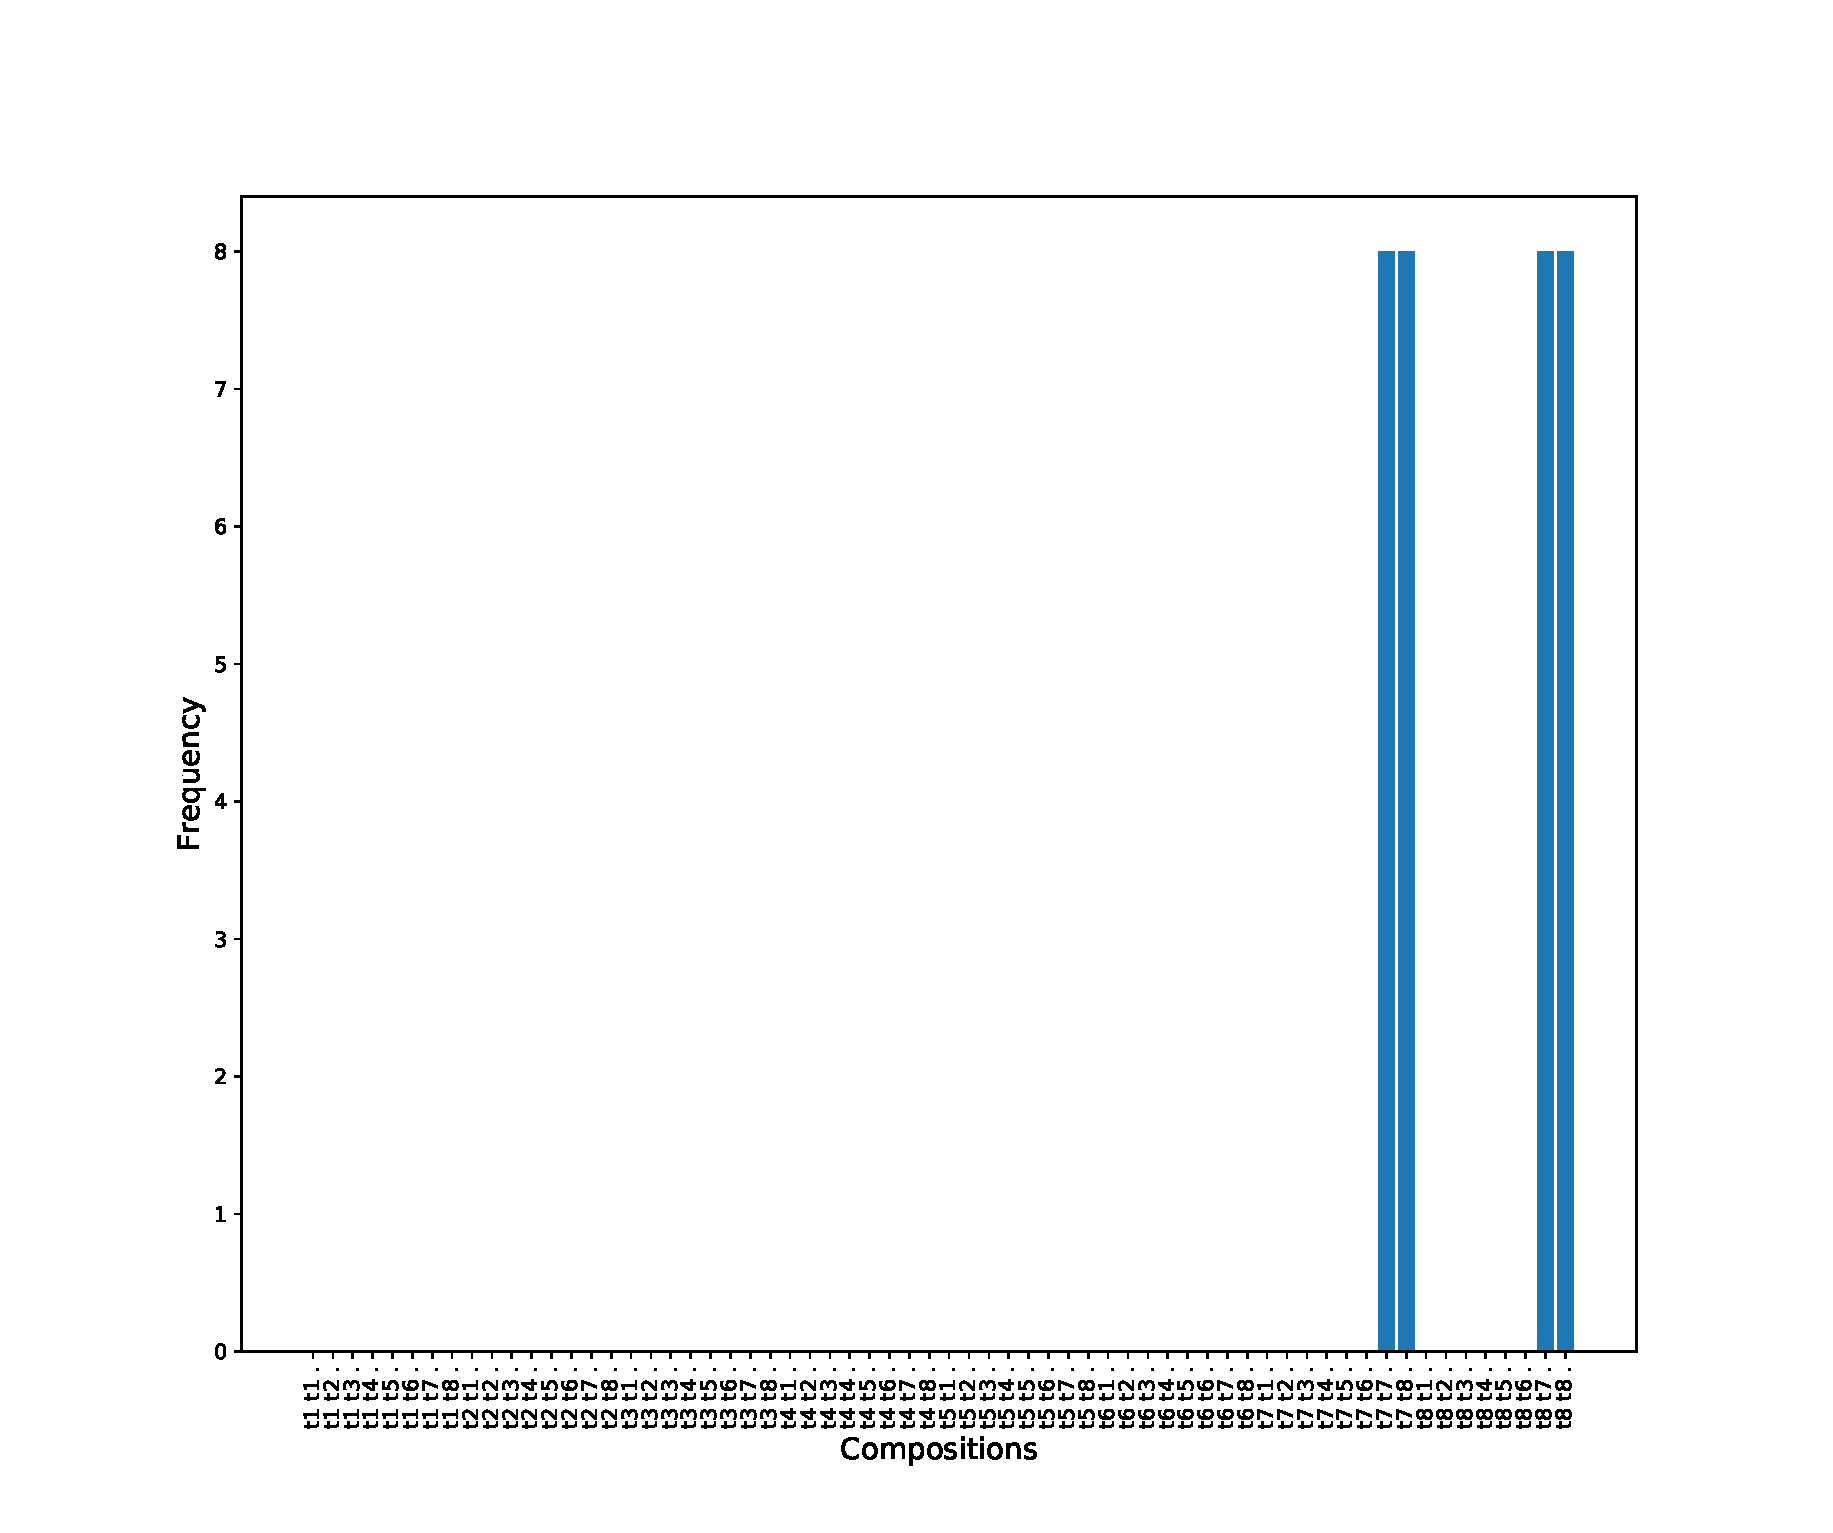
\includegraphics[width=0.95\linewidth]{./figs/lookup/new_compositions-eps}
		\fi
		\caption{New Compositions}\label{fig:new_comp}
	\end{subfigure}
	\caption{Data distribution of train and test sets}\label{fig:all_data}
\end{figure}
%, trim={15mm, 5mm, 35mm, 15mm}, clip
In accordance with the data split described above I present the distribution of all compositions in the train and various test sets. It can be seen that the test sets \lq heldout\_tables\rq{} and \lq new\_compositions \rq{} are the most difficult and require zero-shot generalisation owing to their significantly different distribution as compared to \lq train\rq{}.

\subsection{AG Trace}\label{lt:ponder}
As explained in section \ref{pm:ag-ponder} attentive guidance can help in mocking the pondering. For a lookup table composition of the form \lq $((000)t3)t1$\rq{} AG enforces pondering as follows:
\begin{equation}
t1(111) = 100 \qquad t3(000) = 111 \qquad ((000)t3)t1 = 100,
\end{equation}
the composed function is expanded as follows:
\begin{equation}
000\ t3\ t1 = 000\ 111\ 100.
\end{equation}
AG therefore forces the decoder to ponder for two additional steps. The biggest difference from the Pondering in section \ref{bck:ponder} would be that at each pondering step we have an emission, instead of the ponder step being a silent one. The trace for the attentive guidance can be explained as follows:
%and is shown in figure \ref{ag_lt}:
\begin{itemize}
	\item The first step is the copy step where the three bit input to the composition is copied as it is.
	\item After this the tables in the composition are applied sequentially to the three bit input preceding them.
	\item The diagonal trace is meant to capture this sequential and compositional solution of lookup tables. At each step of decoding the model was forced to focus on only that input prompt which results in the correct output for that step.
\end{itemize}


\subsection{Accuracy}
Since the lookup tables can be viewed as nested functions, accuracy of final output of the composition can be an adequate measure of model performance. However since we want to ensure that the model doesn't learn spurious patterns in data to land at an un-compositional solution, we want it to be accurate at each step of the composition. This hierarchical measure of accuracy is a viable test for the compositionality of the network. Therefore in all evaluations \textit{sequence accuracy} is the performance metric of the model.

\subparagraph{Hyperparameters} Based on the hyperparameter grid search conducted by \cite{Hupkes2018} I ran the experiments with the best hyperparameters for both the baseline - a vanilla seq2seq model (RNN cell=GRU, Embedding size=128, Hidden layer size=512, optimizer=Adam \citep{KingmaB14}, learning rate=0.001, attention=pre-rnn \citep{Bahdanau2014}, alignment measure=mlp(section \ref{mtv:attn})) and attentive guidance model (Embedding size=16, Hidden layer size=512, rest of the hyperparameters are same as the baseline).

\subsection{Lookup Tables - Results}
The impact of AG has been tested by making a comparative study of \textit{learned/guided} models and \textit{baseline} models. Both models are a standard seq2seq architecture as explained in section \ref{bck:s2s}. The only difference between a guided model and baseline is the presence of the extra attention loss term (equation \ref{eqn:ag}) along with the cross-entropy loss between predictions and targets. I sampled five different train and test sets and trained baseline and guided models on each one of them to account for stochasticity during different model runs. I present the results of both the models on the different test sets, discuss their zero shot generalization capabilities and end this section with an analysis of the impact of replacing the learned component of attentive guidance with the exact attention target vectors.

\begin{figure}[ht] 
	\begin{subfigure}[b]{0.5\linewidth}
		\centering
		\ifpdf
		\includegraphics[width=0.95\linewidth]{./figs/lookup/baseline-loss-pdf}
		\else
		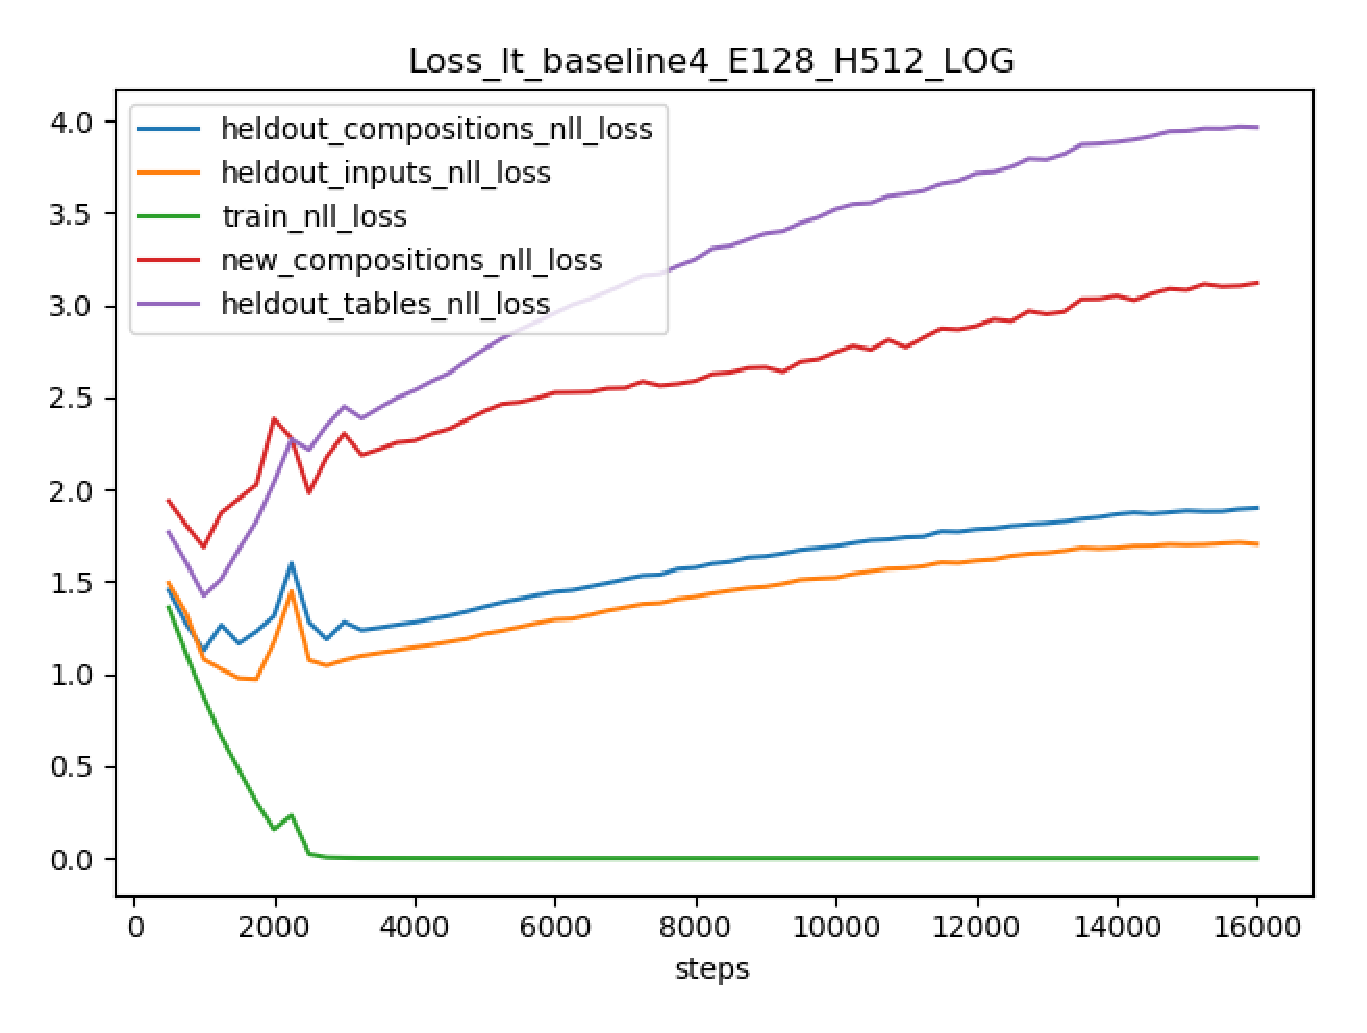
\includegraphics[width=0.95\linewidth]{./figs/lookup/baseline-loss-eps}
		\fi
		\caption{Loss Curves for Baseline} 
		\label{lt_baseline} 
		\vspace{2ex}
	\end{subfigure}%% 
	\begin{subfigure}[b]{0.5\linewidth}
		\centering
		\ifpdf
		\includegraphics[width=0.95\linewidth]{./figs/lookup/learned-loss-pdf}
		\else
		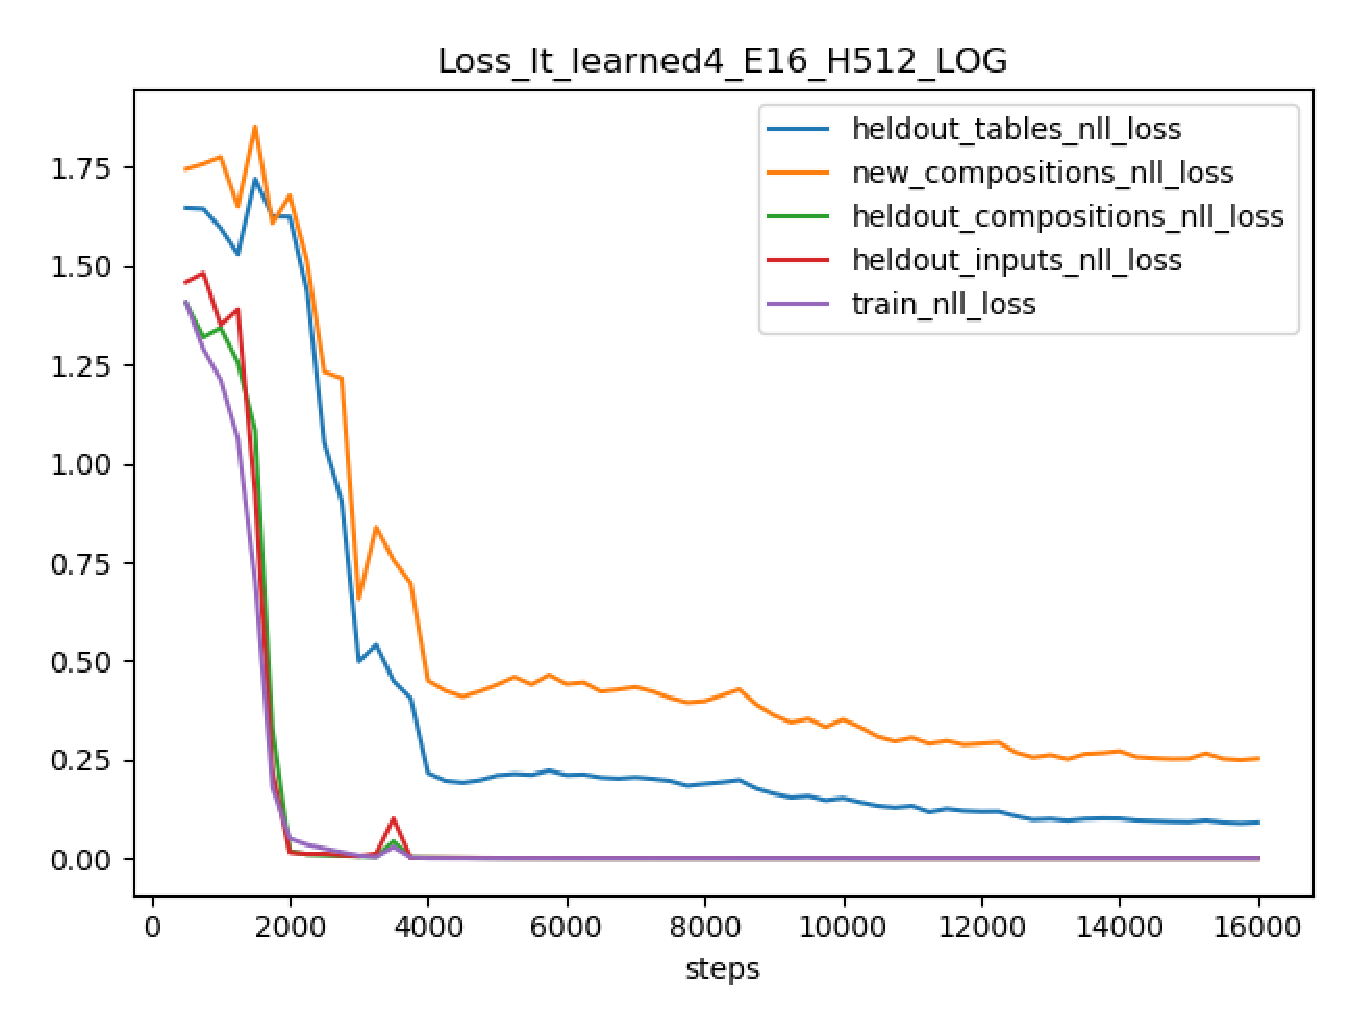
\includegraphics[width=0.95\linewidth]{./figs/lookup/learned-loss-eps}
		\fi 
		\caption{Loss Curves for Learned} 
		\label{lt_learned} 
		\vspace{2ex}
	\end{subfigure}
	\caption{Learning Curves for Lookup Tables}
	\label{lt_learning_curves}
\end{figure}

\begin{figure}[H]
	\begin{minipage}[t]{0.9\textwidth}
		\centering
		\ifpdf
		\includegraphics[width=\linewidth,keepaspectratio=true]{./figs/lookup/lt-acc-pdf}
		\else
		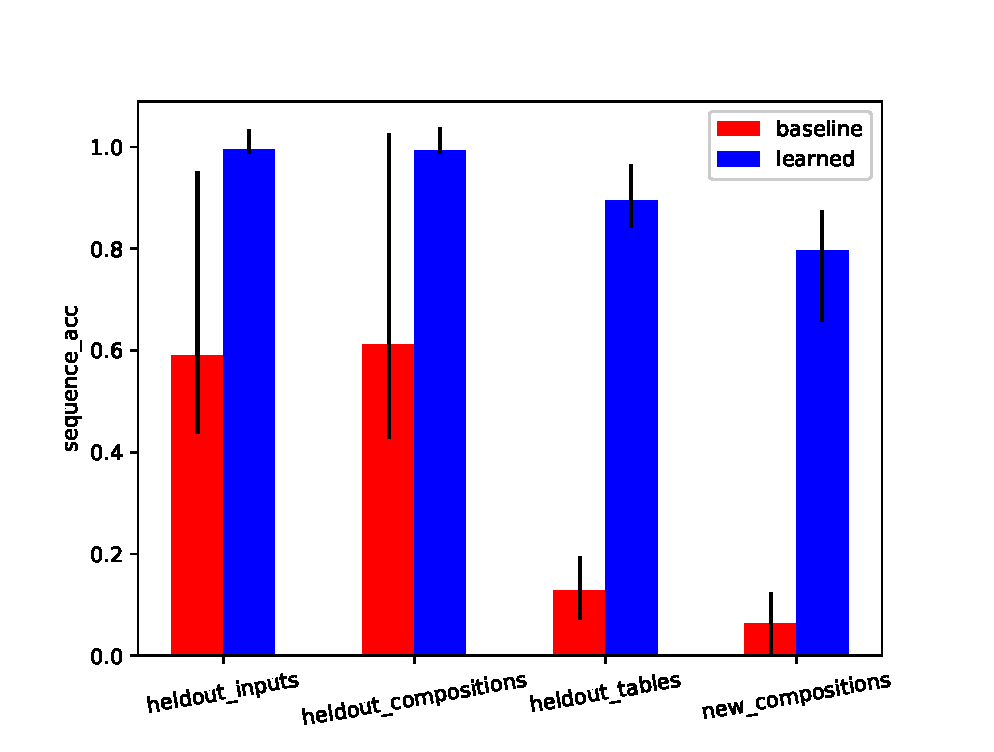
\includegraphics[width=\linewidth,keepaspectratio=true]{./figs/lookup/lt-acc-eps}
		\fi
		\caption{\small Average Sequence Accuracies. Error bars indicate maximum and minimum values achieved by the models.}
		\label{res:lt-acc}
	\end{minipage}
\end{figure}

Focusing on the loss development in the case of baseline (figure \ref{lt_baseline}) and comparing it to the loss development in the case of guided model (figure \ref{lt_learned}) it can be easily concluded that attentive guidance offsets overfitting which is exhibited by the baseline on all the test sets. Further guided models converge much faster in comparison to the baseline models. Despite overfitting on the test sets, the baseline models perform reasonably well above chance level (which stands at 0.2\% for this task) on the \textit{heldout inputs} and \textit{heldout compositions} test splits. However, in contrast to the approximately 60\% accuracy achieved by the baseline of these test sets, the guided model achieves over 99\% i.e they outperform the baseline by 65\%. As we move towards more difficult datasets viz. \textit{heldout tables} and \textit{new compositions} which require zero shot generalization the performance of baseline model progressively deteriorates. Guided models however still manage to achieve 90\% and 80\% sequence accuracy respectively on these datasets. 


\begin{figure}[ht] 
	\begin{subfigure}[b]{0.5\linewidth}
		\centering
		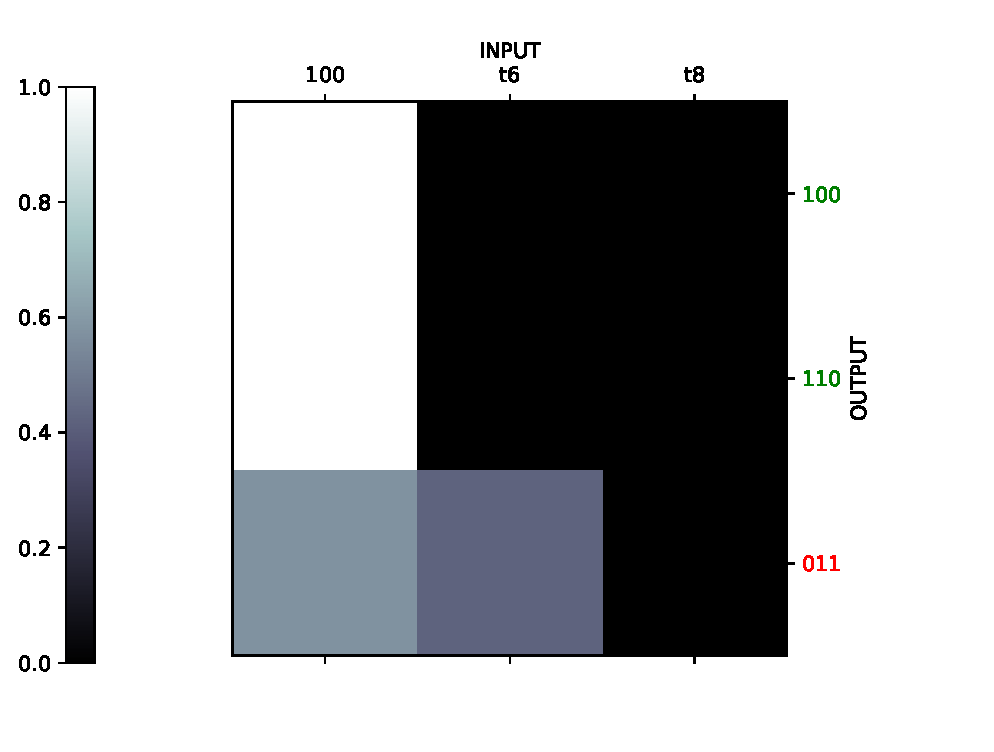
\includegraphics[width=0.95\linewidth]{./figs/lookup/attn/baseline1-eps}
		\caption{Heldout Tables} 
		\label{bs_attn1} 
		\vspace{2ex}
	\end{subfigure}%% 
	\begin{subfigure}[b]{0.5\linewidth}
		\centering
		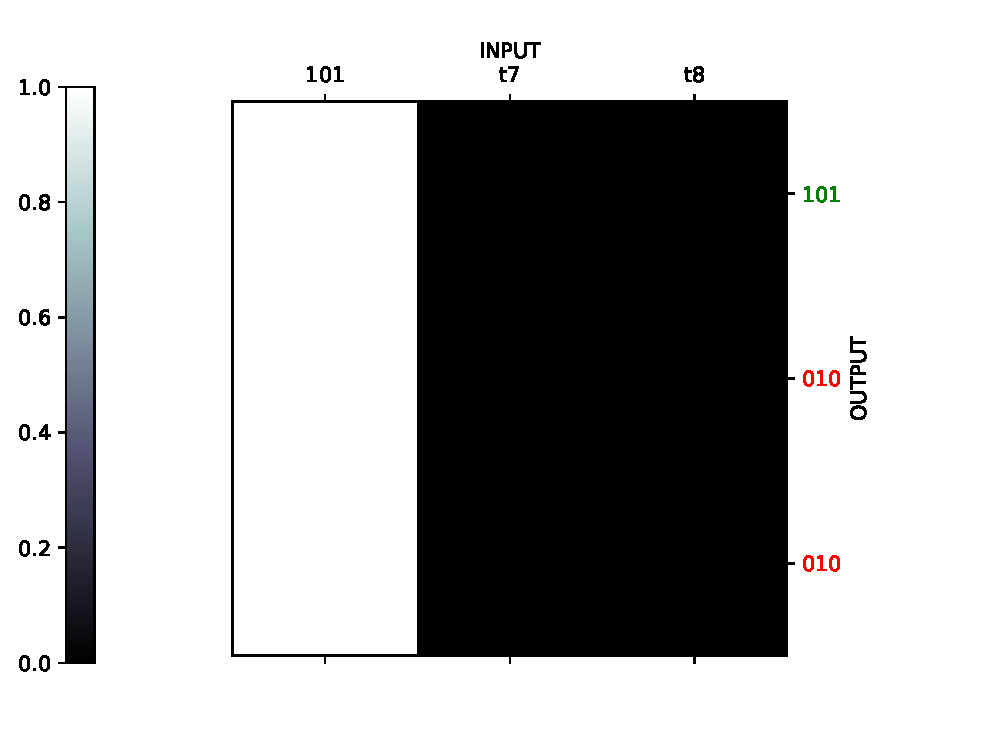
\includegraphics[width=0.95\linewidth]{./figs/lookup/attn/baseline2-eps}
		\caption{New Compositions} 
		\label{bs_attn2} 
		\vspace{2ex}
	\end{subfigure}
	\caption{Attention plots for baseline model.}
	\label{bs_attn}
\end{figure}

\begin{figure}[H] 
	\begin{subfigure}[b]{0.5\linewidth}
		\centering
		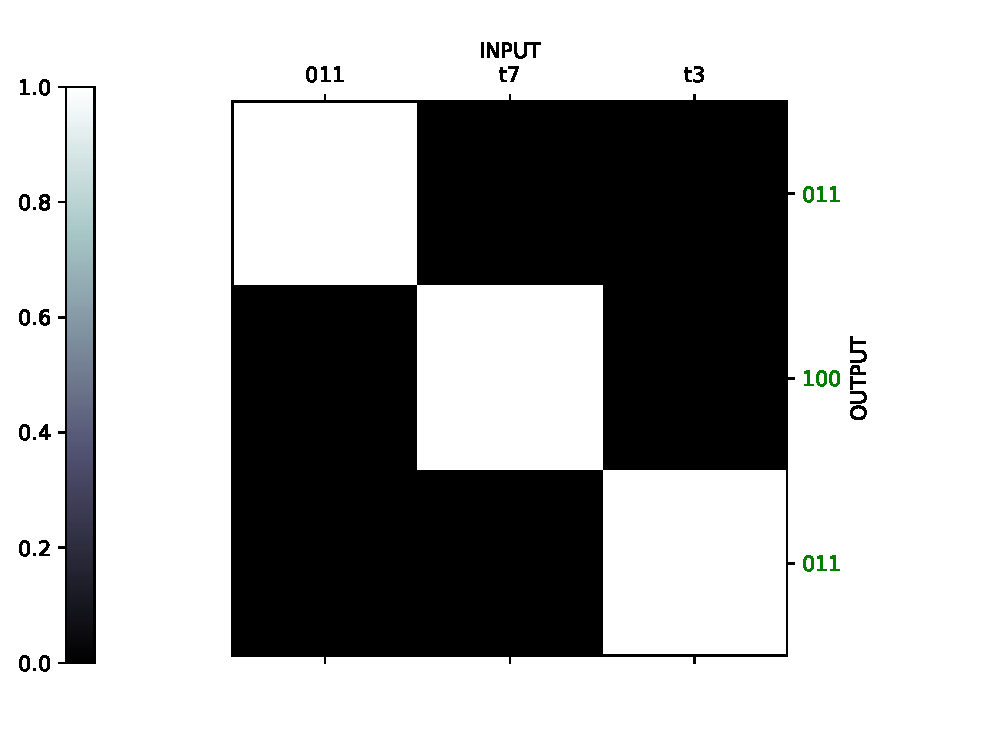
\includegraphics[width=0.95\linewidth]{./figs/lookup/attn/learned1-eps}
		\caption{Heldout Tables} 
		\label{lrn_attn1} 
		\vspace{2ex}
	\end{subfigure}%% 
	\begin{subfigure}[b]{0.5\linewidth}
		\centering
		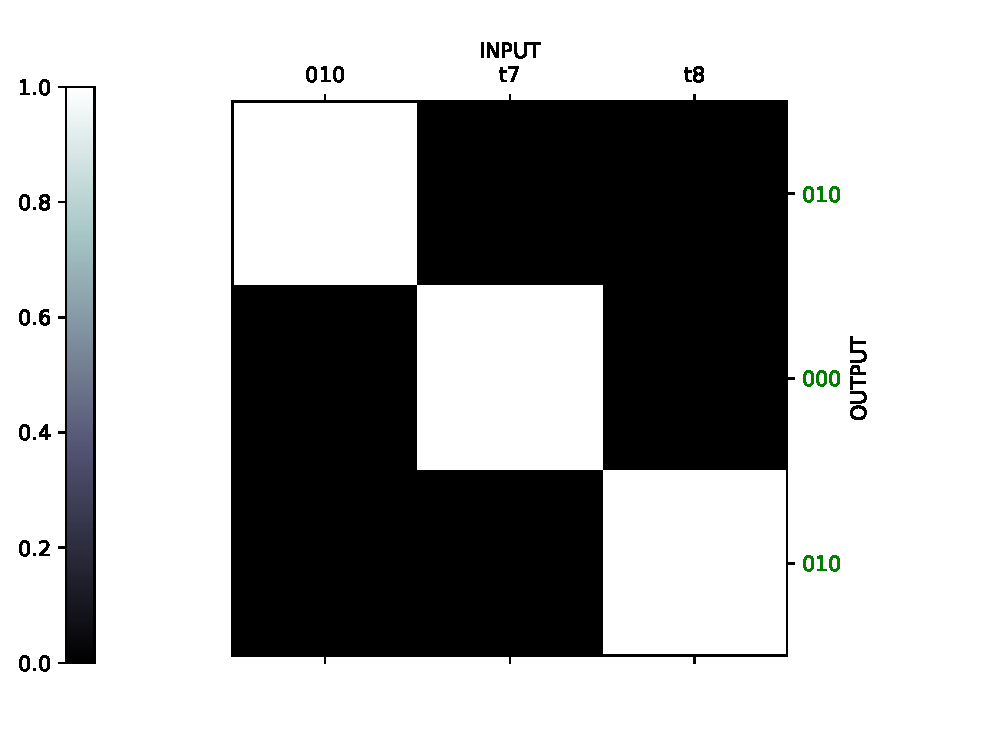
\includegraphics[width=0.95\linewidth]{./figs/lookup/attn/learned2-eps}
		\caption{New Compositions} 
		\label{lrn_attn2} 
		\vspace{2ex}
	\end{subfigure}
	\caption{Attention plot for guided model.}
	\label{lrn_attn}
\end{figure}

\subparagraph{Analysis of Attention:} One of the most salient features of attention based seq2seq models (section \ref{mtv:attn}) is that it is easy to visualize the attention vectors generated by the decoder, thereby making the model interpretable to some degree. Figure \ref{bs_attn} shows that the diffused attention in baseline prohibits it from landing on a compositional solution. The green emissions are correct while the red emissions are incorrect at a given decoding step. Therefore in order to arrive at a compositional solution, the model would need to be compositional even at the intermediate steps. This is easily seen by comparing figures \ref{bs_attn2} and \ref{lrn_attn2}.

%From these results of hard guidance it can argued that the current architectural setup of learning attentive guidance via. an attentive loss term in the final cross-entropy loss, might not be optimal. At the same time these results lend string support to the argument that attention is a key component of compositional learning. 

\begin{figure}[H] 
	\begin{subfigure}[b]{0.5\linewidth}
		\centering
		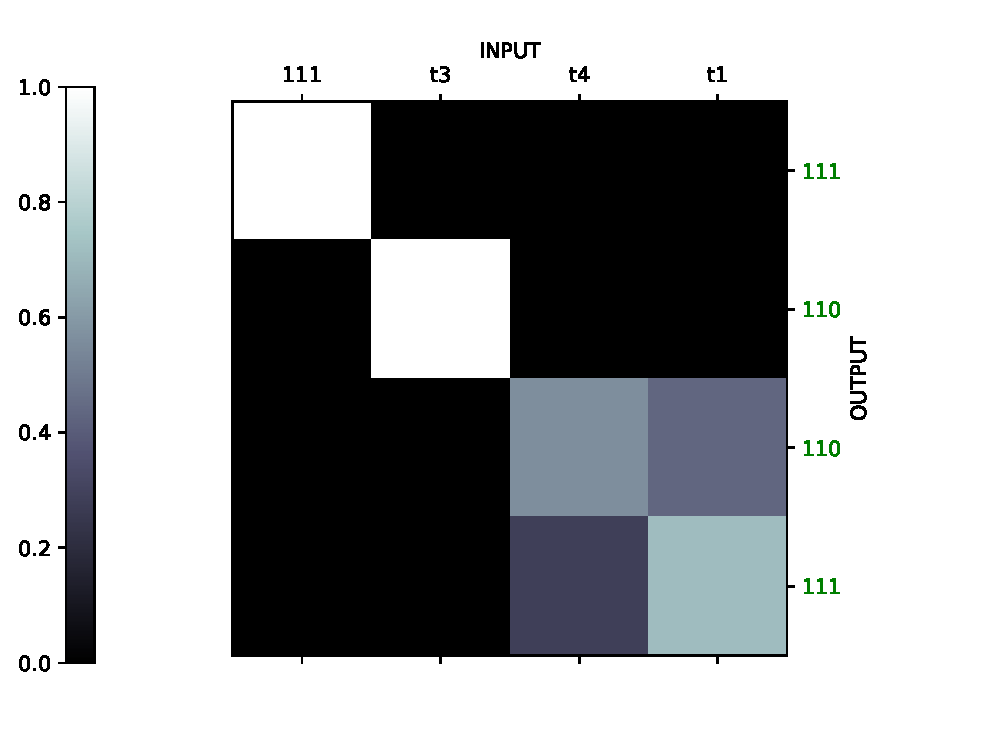
\includegraphics[width=0.95\linewidth]{./figs/lookup/attn/longer2-eps}
		\caption{Attention plot for length=3 heldout composition} 
		\label{attn_longer1} 
		\vspace{2ex}
	\end{subfigure}%% 
	\begin{subfigure}[b]{0.5\linewidth}
		\centering
		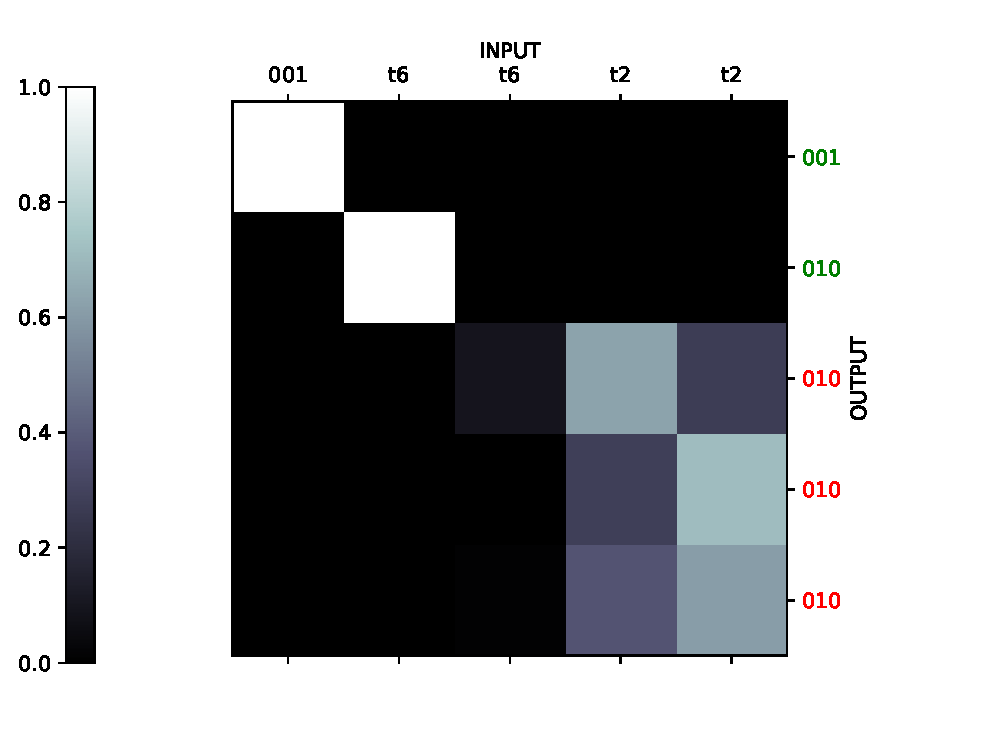
\includegraphics[width=0.95\linewidth]{./figs/lookup/attn/longer1-eps}
		\caption{Attention plot for length = 4 heldout composition} 
		\label{attn_longer2} 
		\vspace{2ex}
	\end{subfigure}
	\caption{Attention plot for longer heldout composition processed by a guided model.}
	\label{attn_longer}
\end{figure}

\begin{figure}[H] 
	\begin{subfigure}[b]{0.5\linewidth}
		\centering
		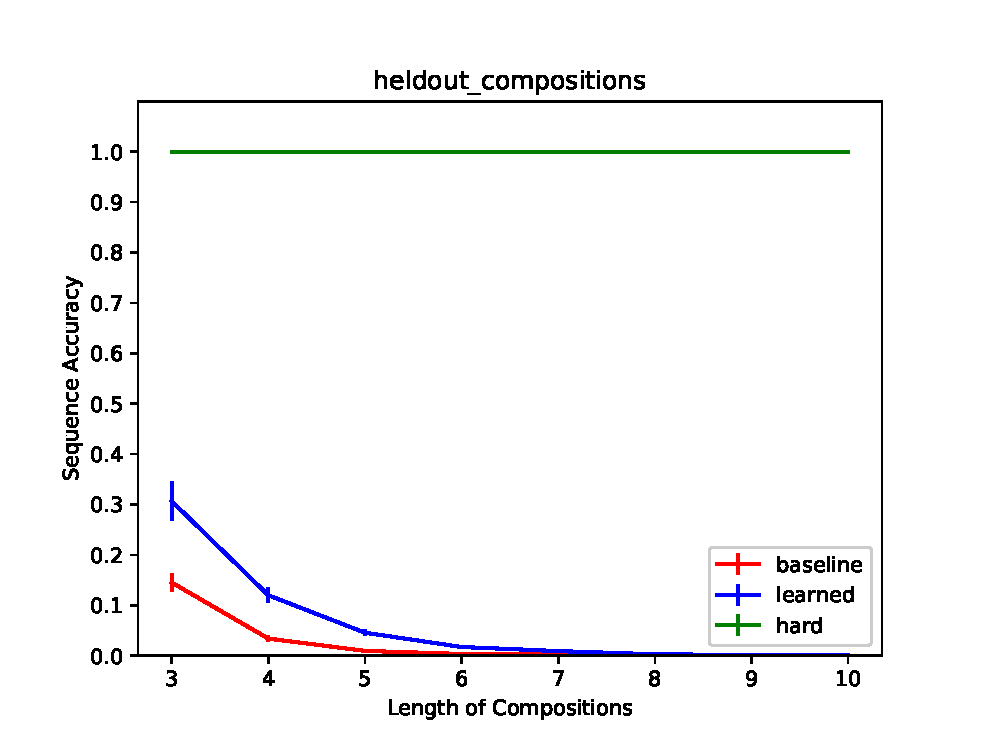
\includegraphics[width=0.95\linewidth]{./figs/lookup/heldout_compositions_eps}
		\caption{Longer Heldout Compositions} 
		\label{lt_longer1} 
		\vspace{2ex}
	\end{subfigure}%% 
	\begin{subfigure}[b]{0.5\linewidth}
		\centering
		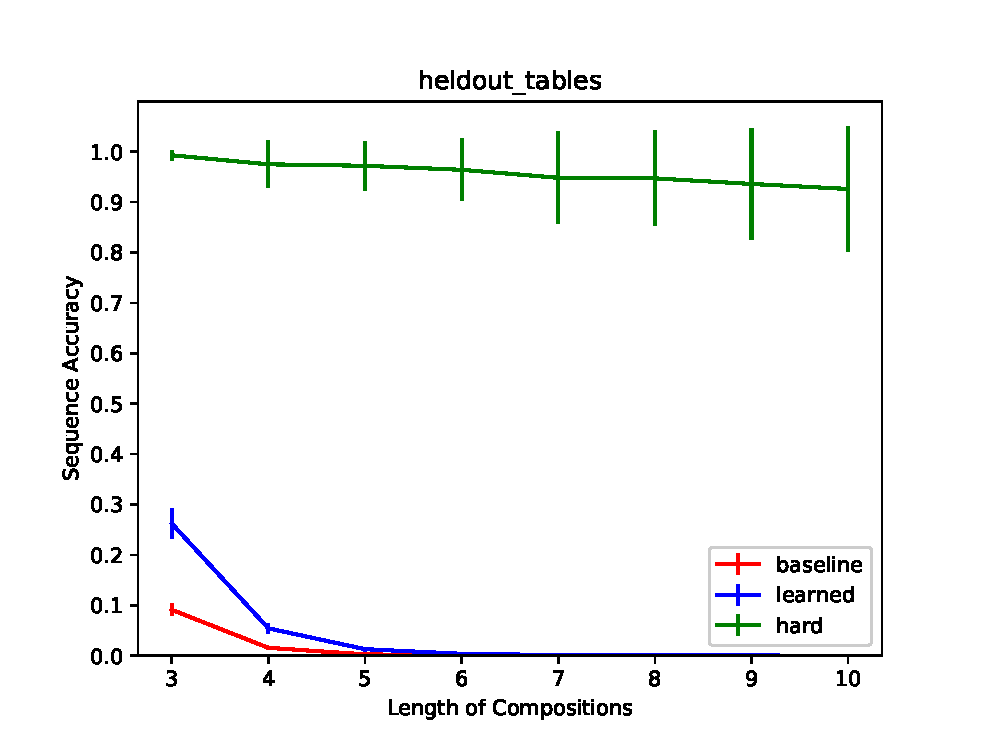
\includegraphics[width=0.95\linewidth]{./figs/lookup/heldout_tables_eps}
		\caption{Longer Heldout Tables} 
		\label{lt_longer2} 
		\vspace{2ex}
	\end{subfigure}
	\caption{Sequence Accuracy for Longer Compositions}
	\label{lt_longer}
\end{figure}

\subparagraph{Longer compositions and hard guidance:} Longer compositions (of length 3 and above) provide the most challenging test case to the guided model and require absolute zero shot generalization from the guided model since it has never been exposed to a sample of length 3 or above. Looking at the attention plots of figure \ref{attn_longer}, we see the guided model now exhibiting the same diffused attention pattern which was the characteristic of baseline attention in figure \ref{bs_attn}. Unsurprisingly the performance of the guided models on longer compositions declines rapidly (it is still higher than baseline) as can be seen from figure \ref{lt_longer}.
However this observation led to experiments with \textit{hard guidance}. Hard guided model remove the need for learning the correct attention by providing the target attention vector at each decoding step. Therefore hard guidance can give some insight into the source of limitation of attentive guidance. As it turns out models trained with hard guidance gave perfect performance on longer heldout compositions, irrespective of the length of the composition (figure \ref{lt_longer1}). Even for a difficult case such as longer heldout tables, hard guidance exhibited high accuracy which had a small gradient with respect to length of composition.

Having tested AG on a dataset that explicitly enforces compositional solution for generalization, it can be concluded that attentive guidance forces a model to discover a compositional solution. This is owing to the fact that AG was able to generalize to compositions which are significantly different from what the model was trained on. But these compositions could be solved by solving the atomic steps in the composition sequentially. I now test AG on a dataset for which the rules are implicit and require a model to infer them from a training data which is considerably larger in size compared to the lookup table data. 



\section{Symbol Rewriting} \label{datasets:sr}
Introduced by \cite{Weber2018} the symbol rewriting dataset is essentially a probabilistic context free grammar (PCFG). It consists of rewriting a set of input symbols to a set of output symbols based on this grammar. Before proceeding further with the task description, I'll elaborate on PCGFs briefly.

\subparagraph{PCFGs} are the stochastic version of CFGs (Context free grammars) that we encountered in section \ref{flt:ch}. The addition of this stochasticity was motivated by the non-uniformity of words in natural language. Assigning probabilities to production rules, leads to a grammar more in line with the Zipfian distribution of words in natural language \citep{jurafsky2014speech}. A PCFG consists of:

\begin{enumerate}
	\item A CFG $\mathcal{G} = \langle \Sigma, N, S, R \rangle$ where the symbols have the same meaning as defined in section \ref{flt}.
	\item A probability parameter $p(a \rightarrow b) \mid \displaystyle \sum_{a \rightarrow b \mid a \in N} p(a \rightarrow b) = 1 $ 
	\item Therefore, the probabilities associated with all the expansion rules of a given non-terminal should sum up to 1.
\end{enumerate}

\begin{figure}
	\begin{minipage}[ht]{\textwidth}
		\ifpdf
		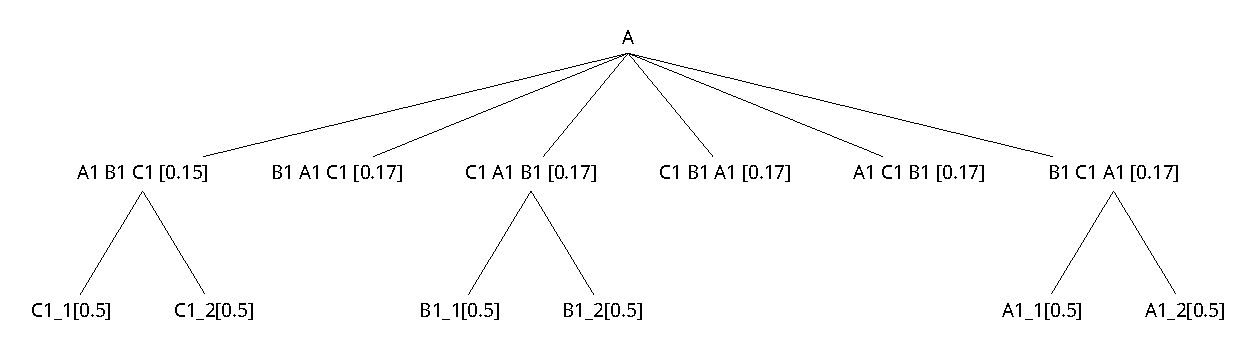
\includegraphics[width=\linewidth,keepaspectratio=true]{./figs/A-pdf}
		\else
		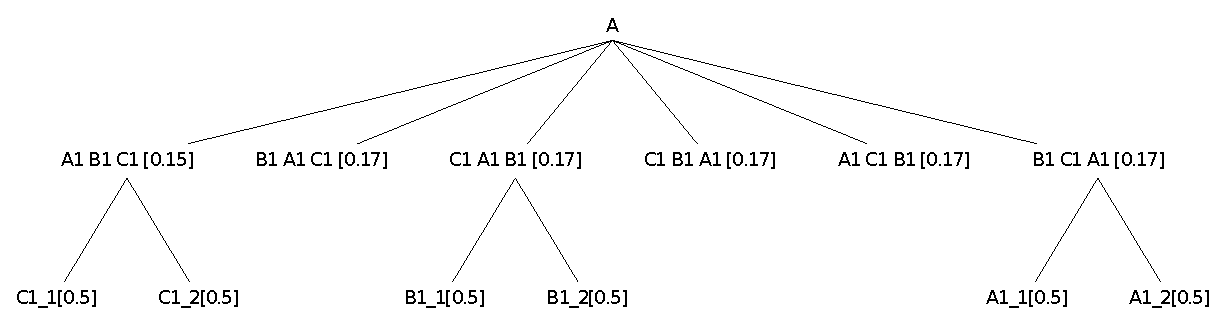
\includegraphics[width=\linewidth,keepaspectratio=true]{./figs/A-eps}
		\fi
		\caption{\small Parse Tree for one Input Symbol. The final symbols (leaf nodes) are shown just once with respect to their parent nodes for clarity.}
		\label{parse-tree}
	\end{minipage}
\end{figure}

The parse tree shown in figure \ref{parse-tree} illustrates the production rule for one input symbol. The grammar consists of 40 such symbols each following similar production rules. \cite{Weber2018} showed using this dataset that seq2seq models are powerful enough to learn some structure from this data and generalize on a test set which was drawn from the same distribution as the training set. They posit that given the simplicity of the grammar it should be possible to generalize to test sets (with some hyperparameter tuning) whose distribution is markedly different from the training distribution while still conforming to the underlying grammar. They however show that this indeed \textbf{is not} the case.

\subsection{Data Structure}
The data-splits as furnished \citep{Weber2018} consists of a training data and different test cases which are non-exhaustive and created by sampling randomly from all possible i/o pairs as described by the PCFG. The different test sets are created to ascertain if the seq2seq models actually understand the underlying grammar from the training data or simply memorize some spurious structure from the training distribution. For hyperparameter tuning, a validation set which is an amalgamation of random samples from all the different test sets, is used. The details of the different data splits are presented below. Examples from each split and the size of each split are presented in table \ref{sr:stats}
\begin{enumerate}
	\item \textbf{train} consists of 100000 pairs of input output symbols with input string length ranging between $\langle$ 5 and 10 $\rangle$. Output string length is therefore between $\langle$ 15 and 30 $\rangle$. A crucial feature of this set is that no symbol is repeated in a given input string.
	\item \textbf{standard test} consists of samples drawn from the same distribution as the training set.
	\item \textbf{repeat test} includes input strings where repetition of symbols is allowed.
	\item \textbf{short test} includes input strings which are shorter in length as compared to the input strings in the training data. The input string length ranges between $\langle$ 1 and 4 $\rangle$.
	\item \textbf{long test} consists of input sequences of lengths in the range $\langle$ 11 and 15 $\rangle$.
\end{enumerate}

\begin{table}[ht]
	\centering
	\begin{tabular}{l|lc}
		& Example & Size\\
		\hline
		train & HS E I G DS  & 100000 \\
		standard test & LS KS G E C P T & 2000 \\
		repeat & I I I I I I MS & 2000 \\
		short & M I C & 2000 \\
		long & Y W G Q V I FS GS C JS R B E M KS & 2000 \\
	\end{tabular}
	\caption{Symbol Rewriting Splits}
	\label{sr:stats}
\end{table}

The datasets \textit{repeat, short and long} come from distributions which are different from the training distribution on which the model has learned the data structure. It is expected of a compositional learner that given the sufficient size of the training data it would be able to infer a pattern which is close to the underlying PCFG and therefore generalize of the test sets which comes from different distributions but have the same underlying structure.

\subsection{AG Trace}\label{sr:trace}
Every input symbol leads to three emissions in the output sequence and each output symbol is generated by exactly one input symbol. Therefore, for every emission in the output sequence the index of the input symbol responsible for the emission, is the trace. For every input there are three decoding steps and for all the three steps the decoder should attend to that particular input.


\subsection{Accuracy}\label{sr:acc_desc}
Given the probabilistic nature of the symbol rewriting dataset it is not difficult to reason that sequence accuracy wouldn't be the ideal performance metric for this task. For instance A $\rightarrow$ A1\_1 B1\_2 C1\_1 and A $\rightarrow$ A1\_2 B1\_1 C1\_2 are both valid productions and since the data is probabilistic, the possibility of both the targets in the training data is equally likely. The accuracy of a prediction is evaluated in the following three steps:
\begin{itemize}
	\item Since every input symbol leads to emission of three output symbols, the output length should be $3*(\text{input length})$.
	\item The input vocabulary consists of 40 symbols (A - OS). The output is always a permutation of a three tuple of the form (Aj\_i Bj\_i Cj\_i) with $j=$ index of the corresponding input symbol in the vocabulary and $i \in [1, 2] $. The second check is to ensure that none of the Aj\_i Bj\_i Cj\_i are repeated.
	\item The third check is that the $j$ as described above = index of the corresponding input symbol in the vocabulary.
\end{itemize}
If a prediction passes all these three checks in that order, the accuracy of that prediction is 1 else 0.

\subparagraph{Hyperparameters} Based on the hyperparameter grid search conducted by \cite{Hupkes2018} I ran the experiments with the best hyperparameters for baseline models (RNN cell=GRU, Embedding size=64, Hidden layer size=64, optimizer=Adam \citep{KingmaB14}, learning rate=0.001, attention=pre-rnn \citep{Bahdanau2014}, alignment measure=mlp(section \ref{mtv:attn})) and the guided models (Embedding size=32, Hidden layer size=256, rest of the hyperparameters are same as in baseline). Additionally since the guided models are operating in a larger parameter space as compared to the baseline, I ran baseline models with the same hyperparameters as the guided models to ensure an unbiased comparison between them. Henceforth baselines (Embedding size=64, Hidden layer size=64) and (Embedding size=32, Hidden layer size=256) are referred to as \textit{baseline1} and \textit{baseline2} respectively.

\subsection{Symbol Rewriting - Results}
The experiments were set in accordance with the requirements outlined by \cite{Weber2018} 1) that a model should learn the generalizable structure from the data i.e should infer the PCFG rules and 2) should not learn spurious dependence between input and output lengths. The purpose of \textit{repeat}, \textit{short and long} datasets respectively is to test a model on these requirements. 50 runs for each of the two baselines and the guided model were carried out with different initialization and their results were then averaged. A comparative analysis of the baselines and guided model has been carried out. I conclude this section with an analysis of the effect of hard guidance.

Loss development on each of the 4 test sets, over the course of training as shown in figure \ref{sr-all-loss} brings forth an interesting observation apart from the fact that guided models converge faster than the baselines. Even the guided (or learned) model seems to be overfitting to the training. However that is not the case since the data is probabilistic and one input can have multiple outputs. Loss therefore is not the best benchmark for comparing the performance of the three models.

\begin{figure}[ht]
	\begin{subfigure}{0.5\linewidth}
		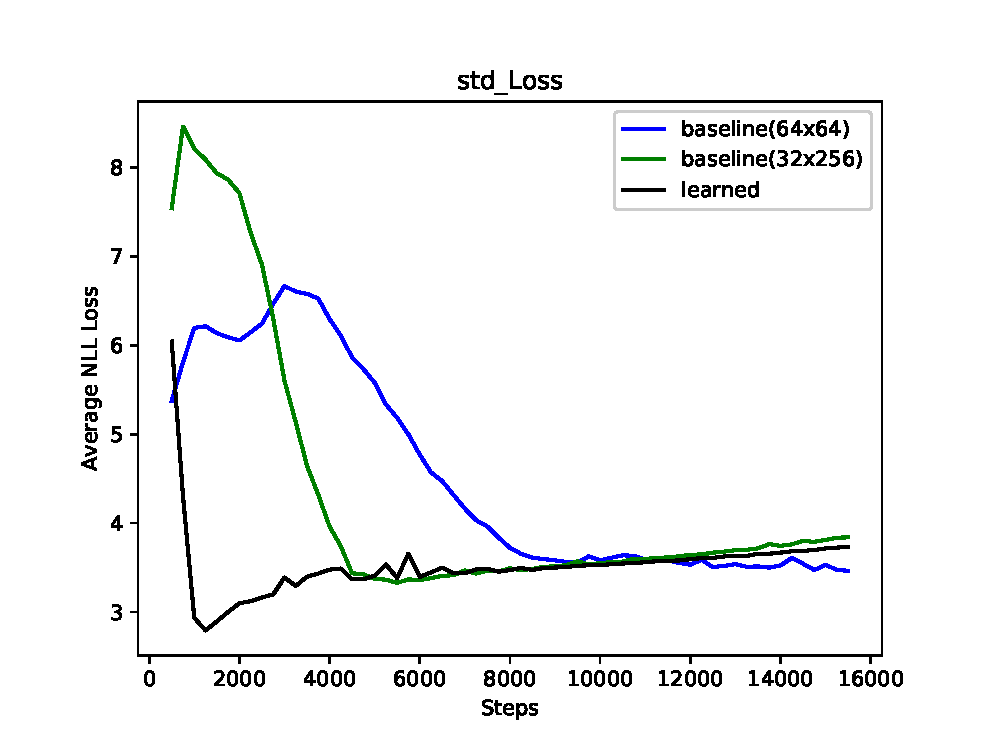
\includegraphics[width=0.95\linewidth]{./figs/sr/std-loss-eps}
		\caption{Standard}\label{std-loss}
	\end{subfigure}
	\begin{subfigure}{0.5\linewidth}
		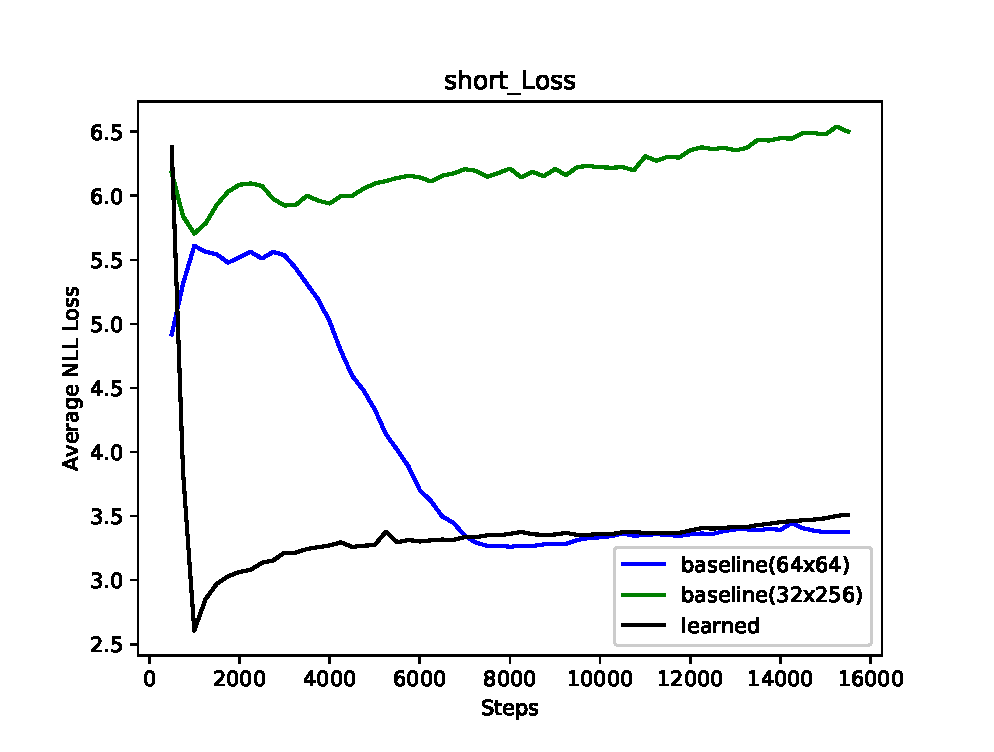
\includegraphics[width=0.95\linewidth]{./figs/sr/short-loss-eps}
		\caption{Short}\label{short-loss}
	\end{subfigure}
	\begin{subfigure}{0.5\linewidth}
		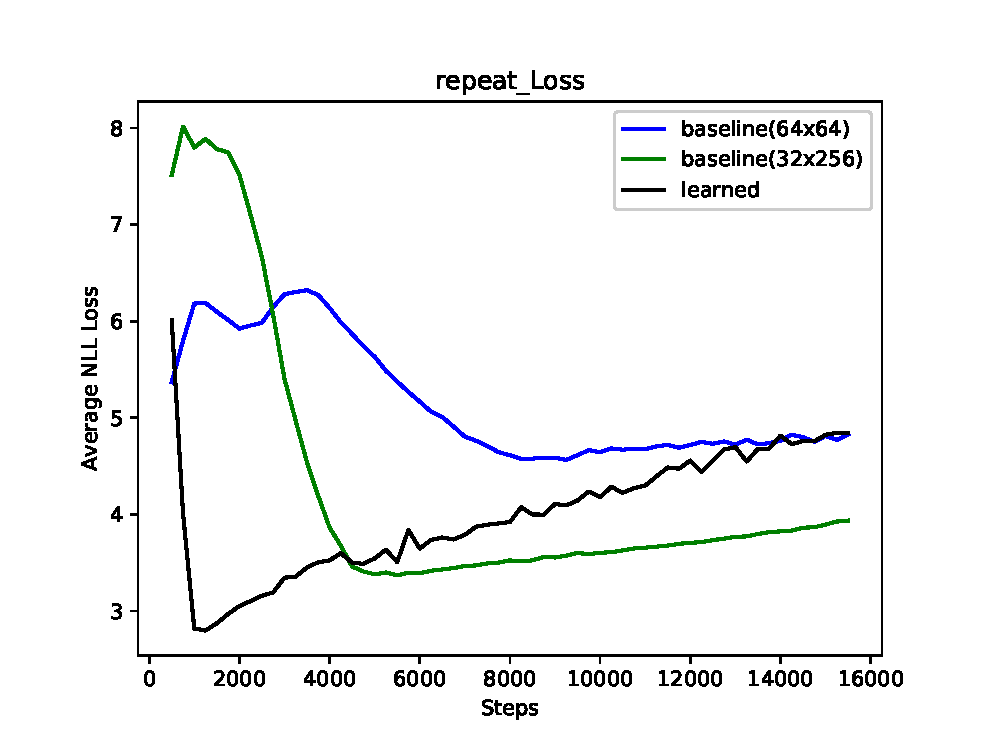
\includegraphics[width=0.95\linewidth]{./figs/sr/repeat-loss-eps}
		\caption{Repeat}\label{repeat-loss}
	\end{subfigure}
	\begin{subfigure}{0.5\linewidth}
		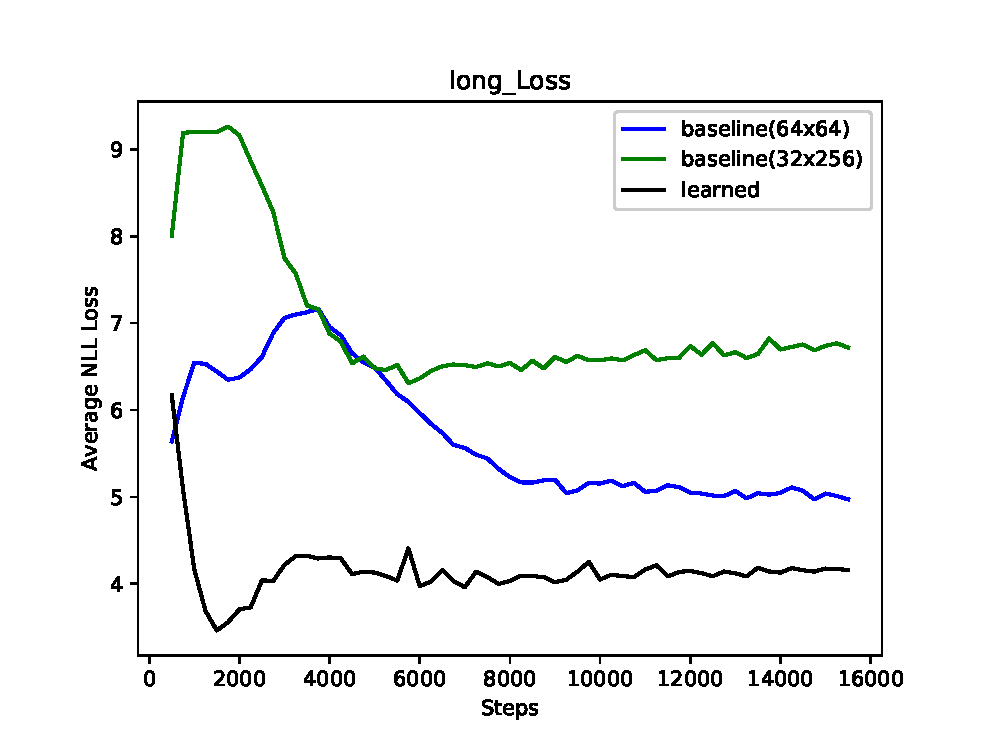
\includegraphics[width=0.95\linewidth]{./figs/sr/long-loss-eps}
		\caption{Long}\label{long-loss}
	\end{subfigure}
	\caption{Average NLL Loss over 50 runs of the selected configuration of all three models}\label{sr-all-loss}
\end{figure}

Focusing now on the accuracy (symbol rewriting accuracy as described in section \ref{sr:acc_desc}), in figure \ref{res:sr-acc}, we can see that our results for baseline are fairly consistent with the ones presented by \cite{Weber2018}. Baseline2 in fact is almost at par with guided model in the standard (same distribution as training data) and repeat(similar to standard with repetition of input symbols allowed) datasets, but it doesn't satisfy the second requirement outlined by the authors in the original paper. It can't generalize to test sets where the input length changes as compared to training data. Baseline1 on the other hand generalizes relatively better to all test sets, although the accuracy is still significantly low in comparison to guided model.

\begin{figure}[H]
	\begin{minipage}[t]{\textwidth}
		\centering
		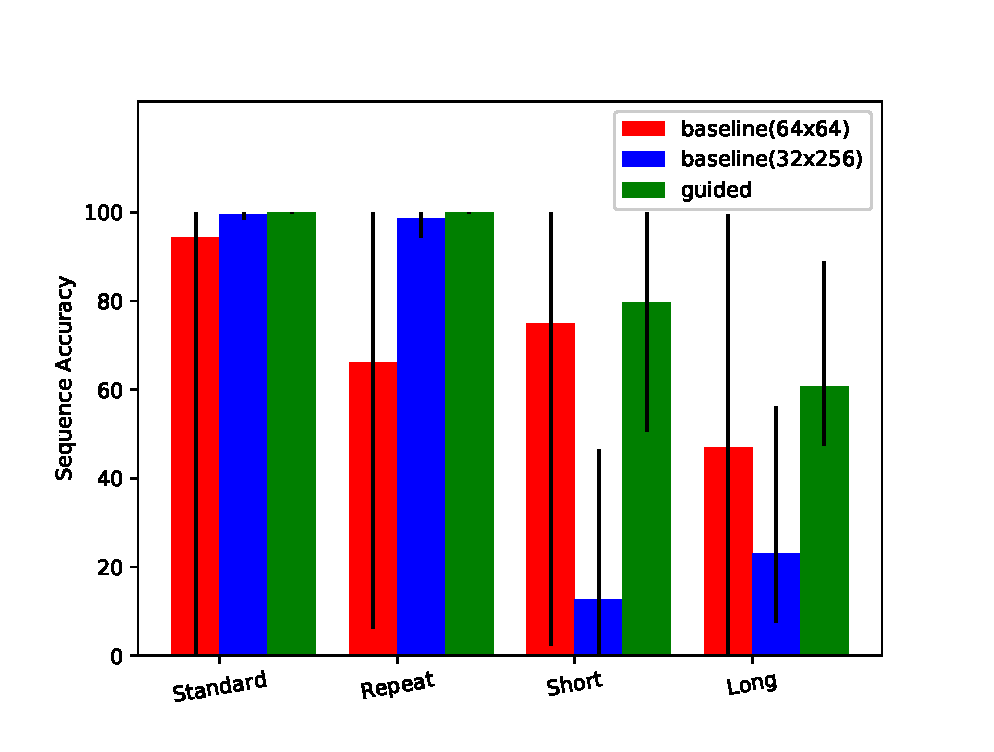
\includegraphics[width=\linewidth,keepaspectratio=true]{./figs/sr/sr-seq-eps}
		\caption{\small Sequence accuracies for symbol rewriting test splits. Error bars indicate maximum and minimum values achieved by the models.}
		\label{res:sr-acc}
	\end{minipage}
\end{figure}

\begin{figure}[ht] 
	\begin{subfigure}[b]{0.5\linewidth}
		\centering
		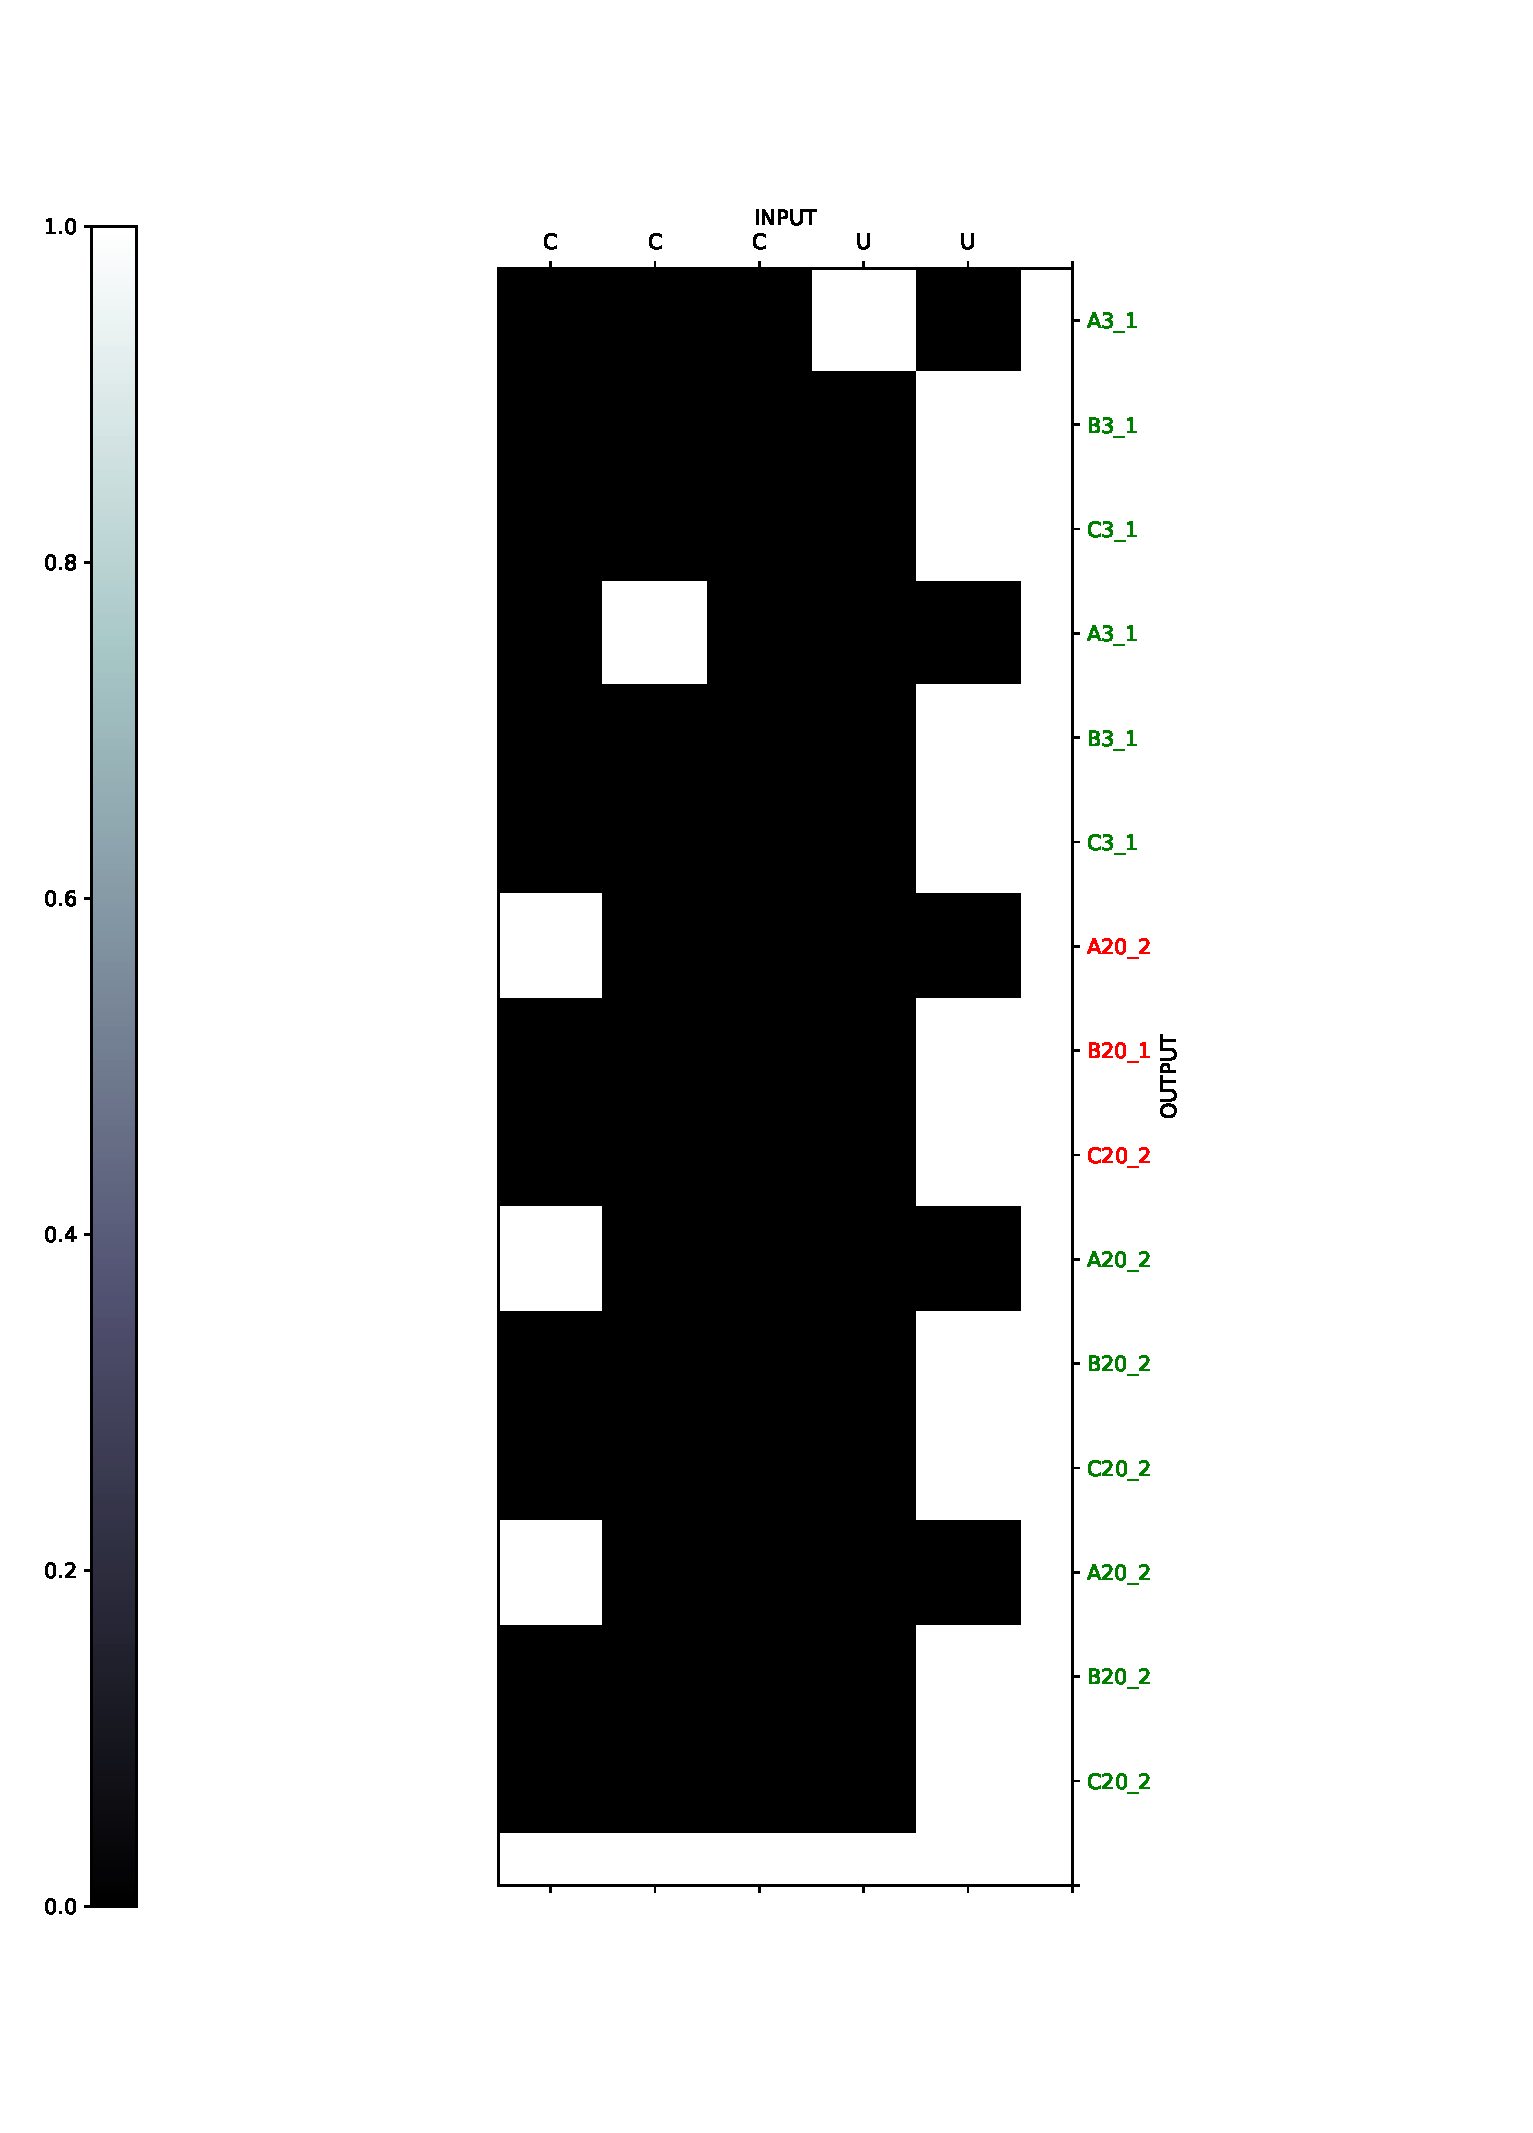
\includegraphics[width=0.95\linewidth]{./figs/sr/attn/baseline-eps}
		\caption{Baseline attention plot for a \lq repeat\rq{} sample} 
		\label{repeat_base} 
		\vspace{2ex}
	\end{subfigure}%% 
	\begin{subfigure}[b]{0.5\linewidth}
		\centering
		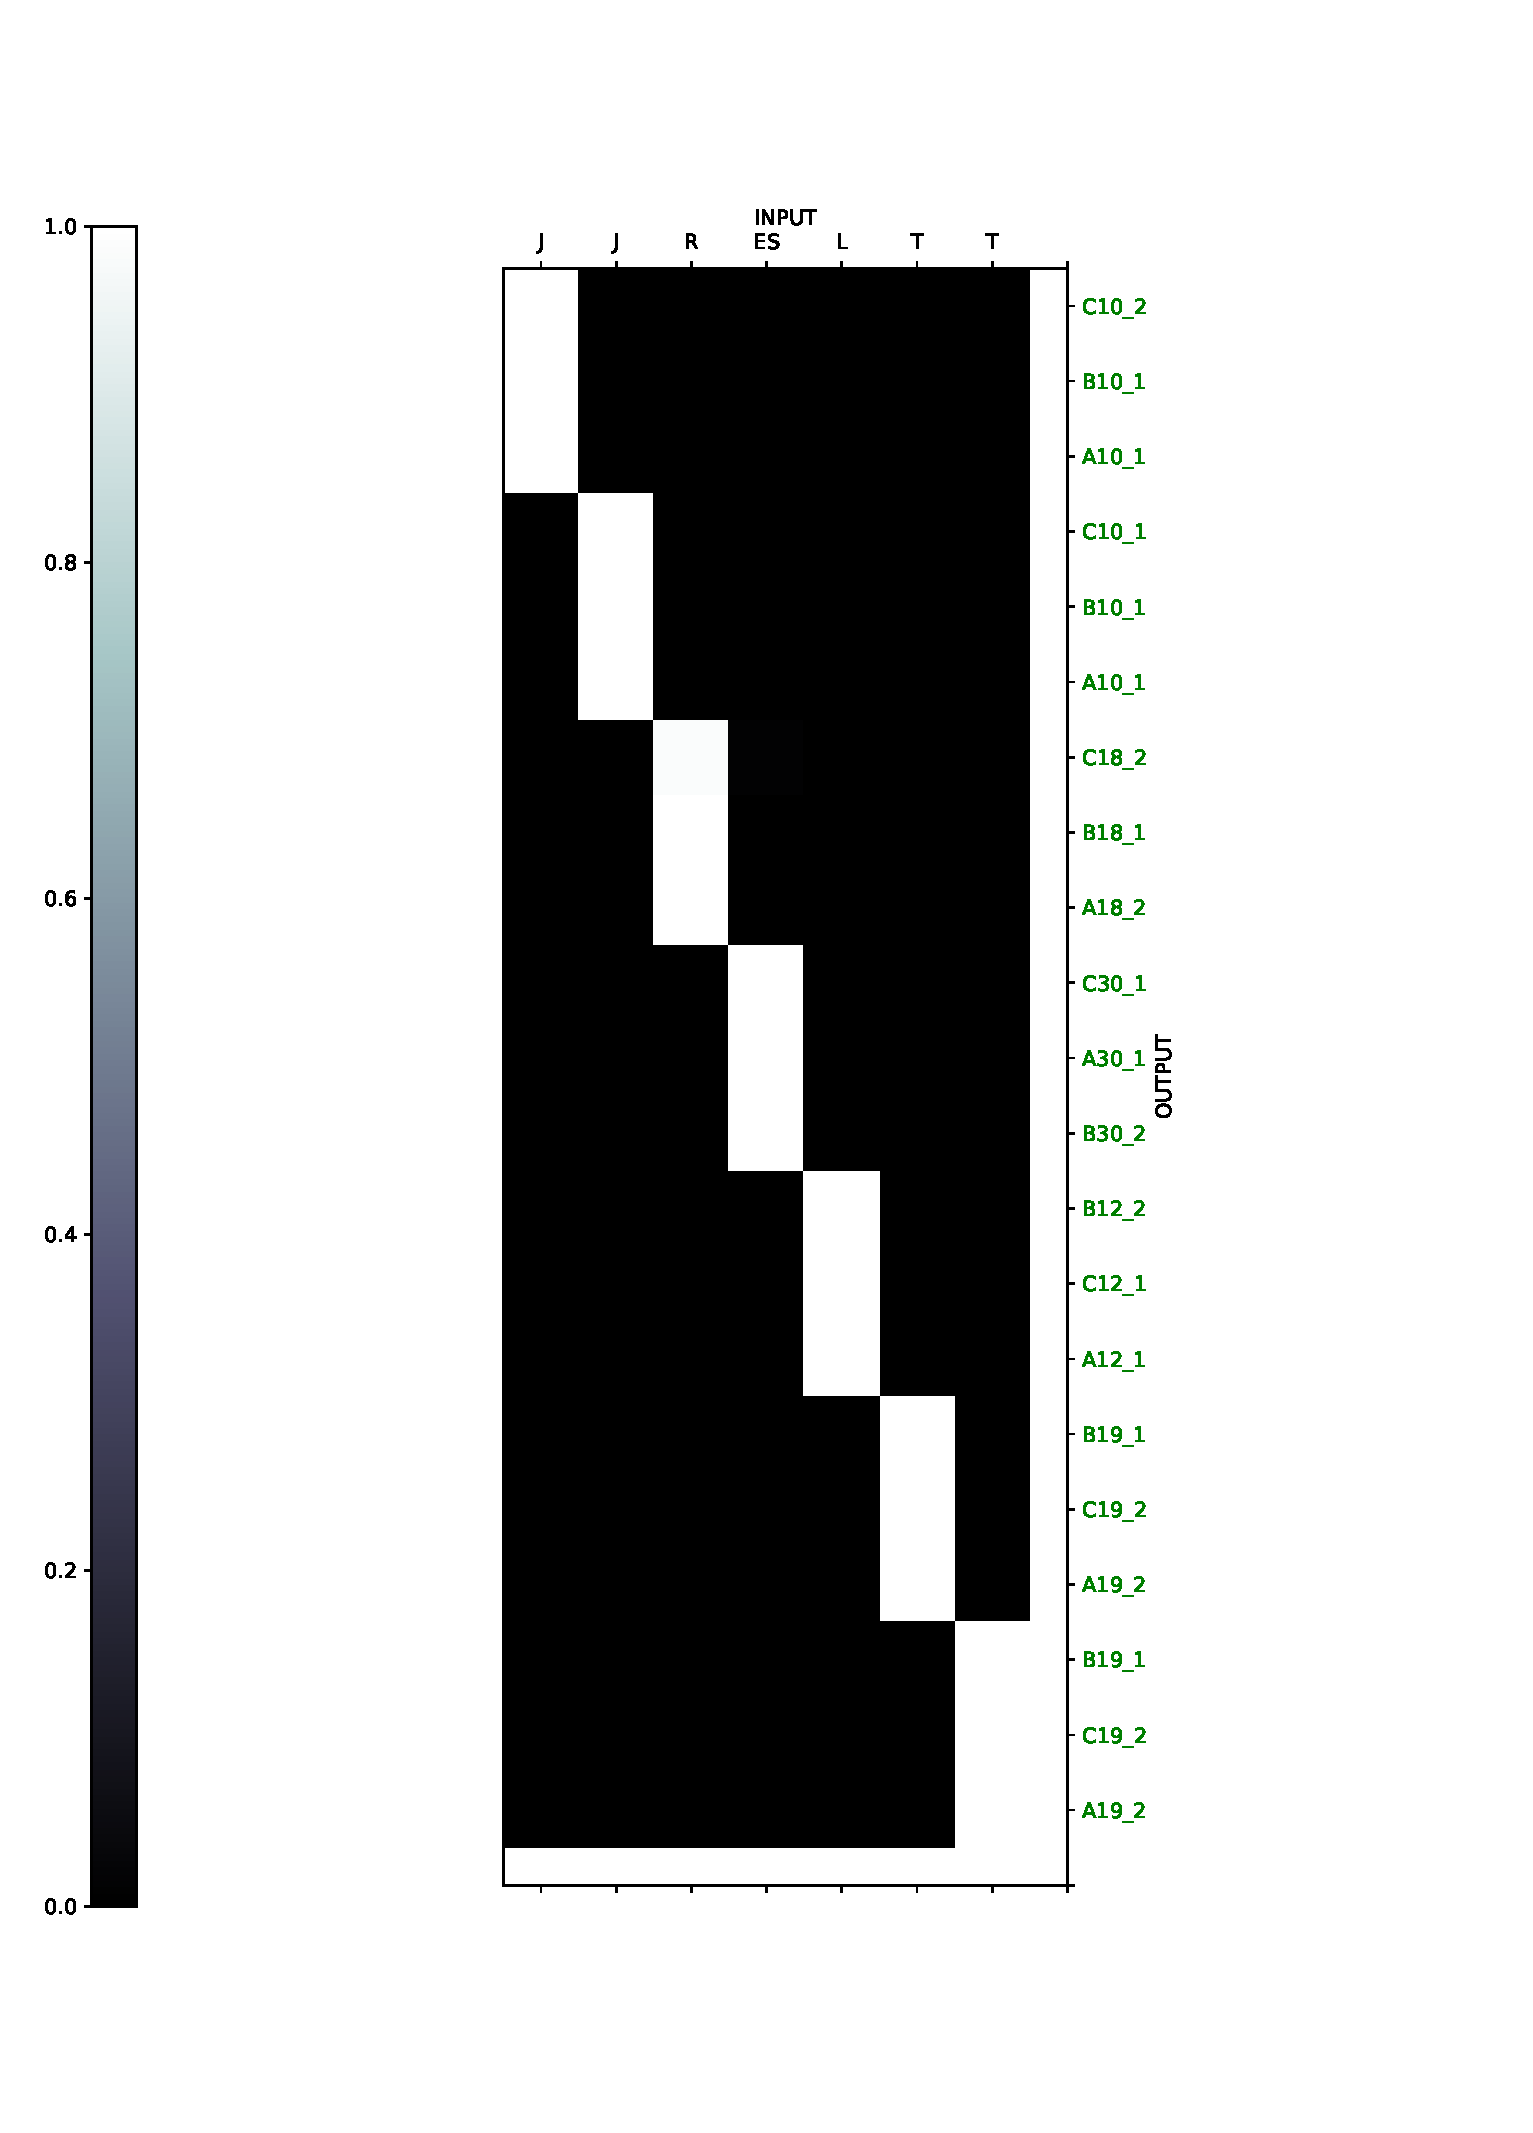
\includegraphics[width=0.95\linewidth]{./figs/sr/attn/guided-eps}
		\caption{AG attention plot for a \lq repeat\rq{} sample } 
		\label{repeat_guide} 
		\vspace{2ex}
	\end{subfigure}
	\caption{Attention plots for symbol rewriting}
	\label{sr_repeat}
\end{figure}
\subparagraph{Analysis of Attention:} Similar to the lookup tables case the baseline attention is diffused over the entire input sequence in stark contrast to the attention of guided models, which have perfectly learned the trace for the symbol rewriting task as outlined in section \ref{sr:trace}. It can be argued by looking at figure \ref{sr_repeat}, that the lack of attentive guidance causes baseline to memorize spurious patterns from the data and that's why after two successful production for the input symbol $C$ it falters when it sees the same symbol for a third time.

\begin{figure}[H]
	\begin{subfigure}{0.5\linewidth}
		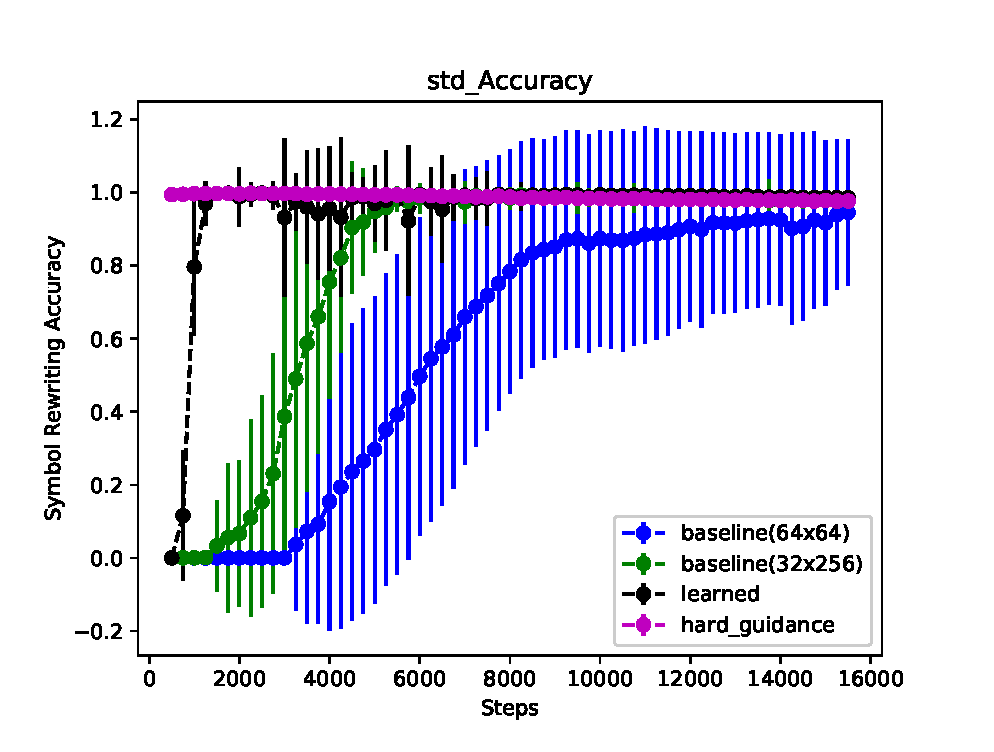
\includegraphics[width=0.95\linewidth]{./figs/sr/std-acc-eps}
		\caption{Standard}\label{std-acc}
	\end{subfigure}
	\begin{subfigure}{0.5\linewidth}
		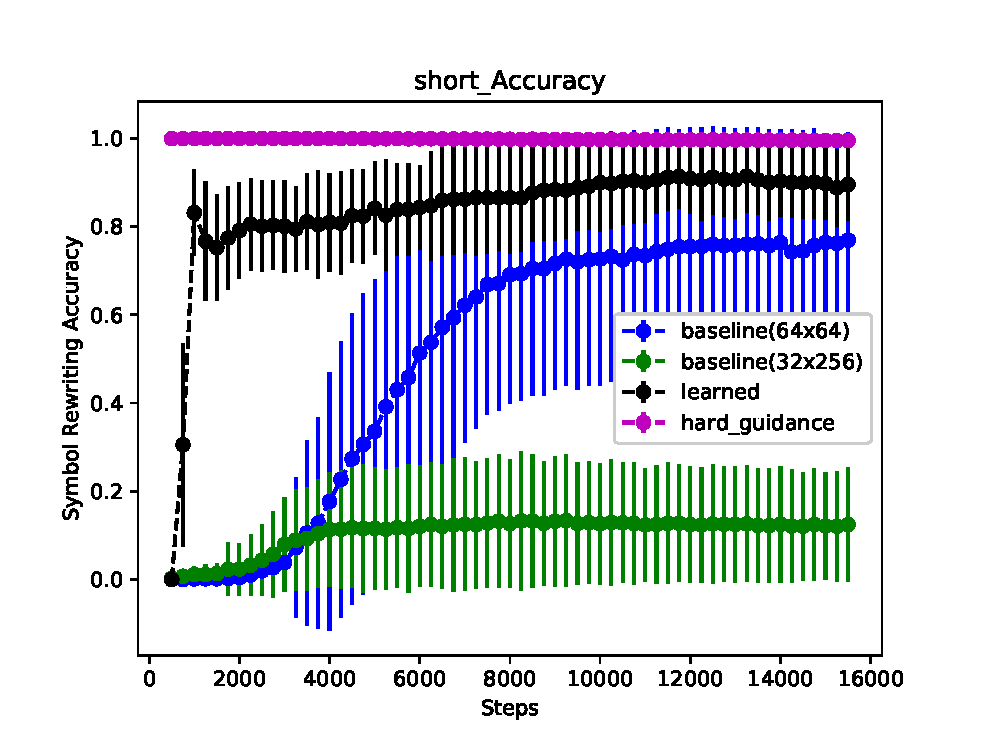
\includegraphics[width=0.95\linewidth]{./figs/sr/short-acc-eps}
		\caption{Short}\label{short-acc}
	\end{subfigure}
	\begin{subfigure}{0.5\linewidth}
		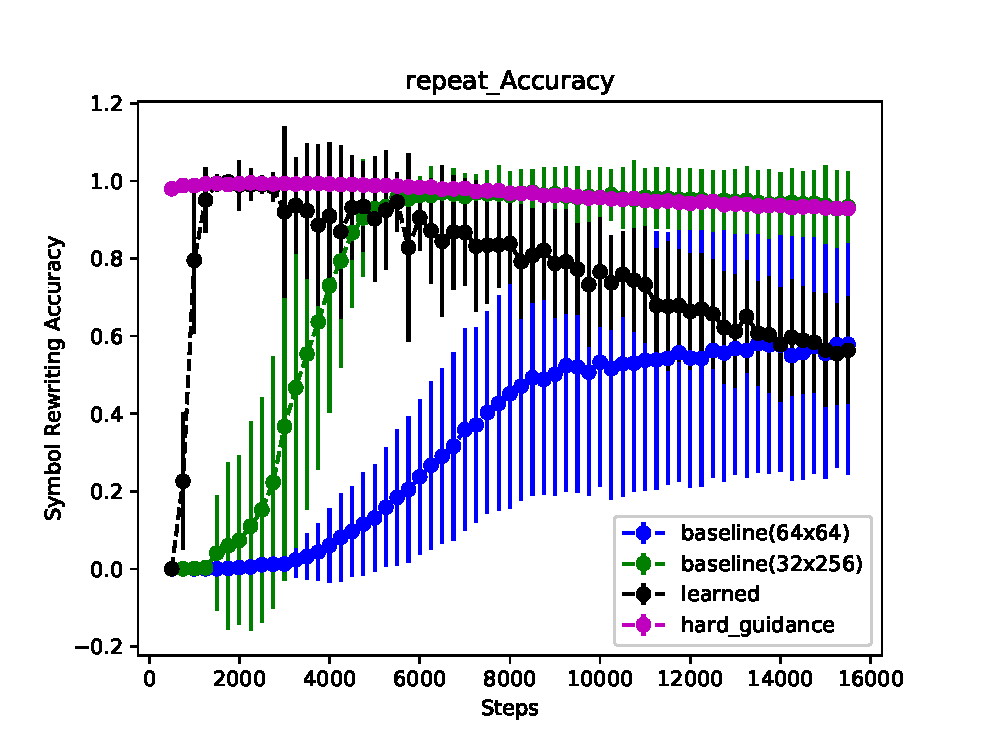
\includegraphics[width=0.95\linewidth]{./figs/sr/repeat-acc-eps}
		\caption{Repeat}\label{repeat-acc}
	\end{subfigure}
	\begin{subfigure}{0.5\linewidth}
		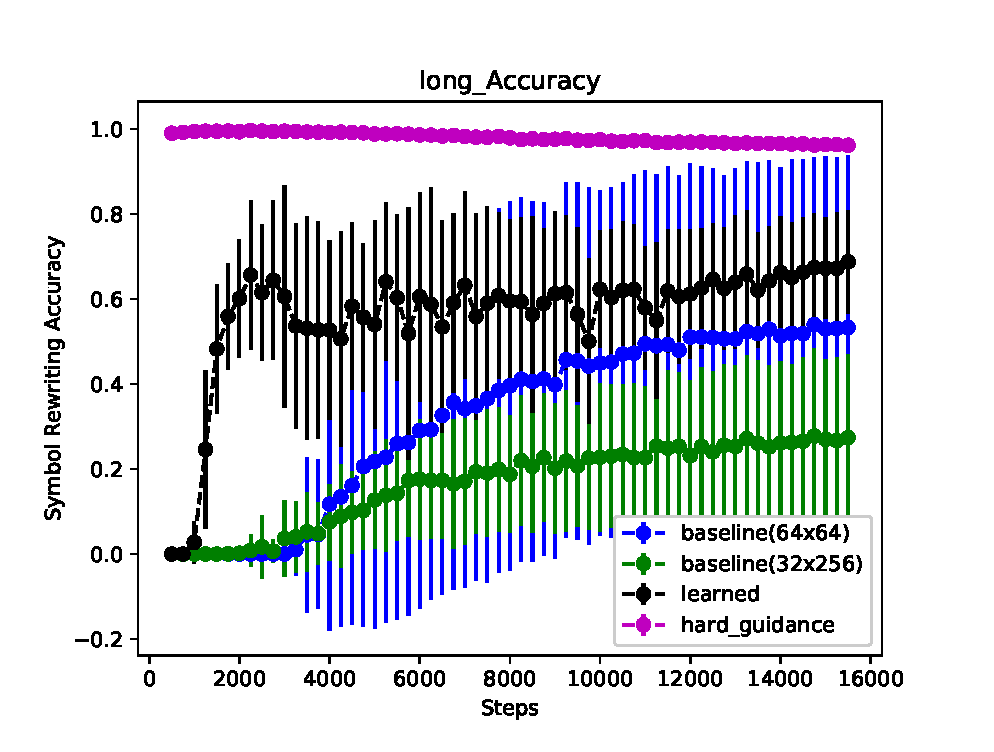
\includegraphics[width=0.95\linewidth]{./figs/sr/long-acc-eps}
		\caption{Long}\label{long-acc}
	\end{subfigure}
	\caption{Average accuracy over 50 runs of the selected configuration of all three models}\label{sr-all-acc}
\end{figure}

\subparagraph{Solving symbol rewriting with hard guidance:} The guided models perform better on the test splits as compared to the baselines and as can be seen from figure \ref{sr-all-acc}, they do so while showing less variance than the baseline models. However they still can't overcome learning the dependencies between the input and output length and this is reflected in their poor performance on the longer test data. Models trained with hard guidance however were able to reach almost perfect accuracy on all the test splits as seen in figure \ref{sr-all-acc}.

\section{Discussion}\label{pm:disc}

This chapter introduced the concept of Attentive Guidance which is a novel concept to \textit{nudge} a seq2seq network in the direction of compositional solutions. The proposed method was tested in two domains, one of which involved sequential application of functions to solve a nested or composed function while the other one required a model to infer the rules of the grammar underlying a dataset in order to be able to generalize to test data which differs significantly from the training data while following the same rules. We saw that hard guidance was actually able to solve both the problems and generalize to unseen test data and this bolsters the argument that attention or more precisely the guidance of it is central to finding compositional solutions. At the same time, the inability of models trained with AG to scale up to complex datasets in a zero shot fashion indicates that the current architecture and the method of learning the guidance via. cross entropy loss isn't optimal and we need to come up with more robust mechanisms to guide attention.